% Options for packages loaded elsewhere
\PassOptionsToPackage{unicode}{hyperref}
\PassOptionsToPackage{hyphens}{url}
\PassOptionsToPackage{dvipsnames,svgnames,x11names}{xcolor}
%
\documentclass[
  letterpaper,
  DIV=11,
  numbers=noendperiod,
  oneside]{scrreprt}

\usepackage{amsmath,amssymb}
\usepackage{iftex}
\ifPDFTeX
  \usepackage[T1]{fontenc}
  \usepackage[utf8]{inputenc}
  \usepackage{textcomp} % provide euro and other symbols
\else % if luatex or xetex
  \usepackage{unicode-math}
  \defaultfontfeatures{Scale=MatchLowercase}
  \defaultfontfeatures[\rmfamily]{Ligatures=TeX,Scale=1}
\fi
\usepackage{lmodern}
\ifPDFTeX\else  
    % xetex/luatex font selection
\fi
% Use upquote if available, for straight quotes in verbatim environments
\IfFileExists{upquote.sty}{\usepackage{upquote}}{}
\IfFileExists{microtype.sty}{% use microtype if available
  \usepackage[]{microtype}
  \UseMicrotypeSet[protrusion]{basicmath} % disable protrusion for tt fonts
}{}
\makeatletter
\@ifundefined{KOMAClassName}{% if non-KOMA class
  \IfFileExists{parskip.sty}{%
    \usepackage{parskip}
  }{% else
    \setlength{\parindent}{0pt}
    \setlength{\parskip}{6pt plus 2pt minus 1pt}}
}{% if KOMA class
  \KOMAoptions{parskip=half}}
\makeatother
\usepackage{xcolor}
\usepackage[left=1in,marginparwidth=2.0666666666667in,textwidth=4.1333333333333in,marginparsep=0.3in]{geometry}
\setlength{\emergencystretch}{3em} % prevent overfull lines
\setcounter{secnumdepth}{5}
% Make \paragraph and \subparagraph free-standing
\ifx\paragraph\undefined\else
  \let\oldparagraph\paragraph
  \renewcommand{\paragraph}[1]{\oldparagraph{#1}\mbox{}}
\fi
\ifx\subparagraph\undefined\else
  \let\oldsubparagraph\subparagraph
  \renewcommand{\subparagraph}[1]{\oldsubparagraph{#1}\mbox{}}
\fi


\providecommand{\tightlist}{%
  \setlength{\itemsep}{0pt}\setlength{\parskip}{0pt}}\usepackage{longtable,booktabs,array}
\usepackage{calc} % for calculating minipage widths
% Correct order of tables after \paragraph or \subparagraph
\usepackage{etoolbox}
\makeatletter
\patchcmd\longtable{\par}{\if@noskipsec\mbox{}\fi\par}{}{}
\makeatother
% Allow footnotes in longtable head/foot
\IfFileExists{footnotehyper.sty}{\usepackage{footnotehyper}}{\usepackage{footnote}}
\makesavenoteenv{longtable}
\usepackage{graphicx}
\makeatletter
\def\maxwidth{\ifdim\Gin@nat@width>\linewidth\linewidth\else\Gin@nat@width\fi}
\def\maxheight{\ifdim\Gin@nat@height>\textheight\textheight\else\Gin@nat@height\fi}
\makeatother
% Scale images if necessary, so that they will not overflow the page
% margins by default, and it is still possible to overwrite the defaults
% using explicit options in \includegraphics[width, height, ...]{}
\setkeys{Gin}{width=\maxwidth,height=\maxheight,keepaspectratio}
% Set default figure placement to htbp
\makeatletter
\def\fps@figure{htbp}
\makeatother
\newlength{\cslhangindent}
\setlength{\cslhangindent}{1.5em}
\newlength{\csllabelwidth}
\setlength{\csllabelwidth}{3em}
\newlength{\cslentryspacingunit} % times entry-spacing
\setlength{\cslentryspacingunit}{\parskip}
\newenvironment{CSLReferences}[2] % #1 hanging-ident, #2 entry spacing
 {% don't indent paragraphs
  \setlength{\parindent}{0pt}
  % turn on hanging indent if param 1 is 1
  \ifodd #1
  \let\oldpar\par
  \def\par{\hangindent=\cslhangindent\oldpar}
  \fi
  % set entry spacing
  \setlength{\parskip}{#2\cslentryspacingunit}
 }%
 {}
\usepackage{calc}
\newcommand{\CSLBlock}[1]{#1\hfill\break}
\newcommand{\CSLLeftMargin}[1]{\parbox[t]{\csllabelwidth}{#1}}
\newcommand{\CSLRightInline}[1]{\parbox[t]{\linewidth - \csllabelwidth}{#1}\break}
\newcommand{\CSLIndent}[1]{\hspace{\cslhangindent}#1}

\KOMAoption{captions}{tableheading}
\makeatletter
\makeatother
\makeatletter
\@ifpackageloaded{bookmark}{}{\usepackage{bookmark}}
\makeatother
\makeatletter
\@ifpackageloaded{caption}{}{\usepackage{caption}}
\AtBeginDocument{%
\ifdefined\contentsname
  \renewcommand*\contentsname{Table of contents}
\else
  \newcommand\contentsname{Table of contents}
\fi
\ifdefined\listfigurename
  \renewcommand*\listfigurename{List of Figures}
\else
  \newcommand\listfigurename{List of Figures}
\fi
\ifdefined\listtablename
  \renewcommand*\listtablename{List of Tables}
\else
  \newcommand\listtablename{List of Tables}
\fi
\ifdefined\figurename
  \renewcommand*\figurename{Figure}
\else
  \newcommand\figurename{Figure}
\fi
\ifdefined\tablename
  \renewcommand*\tablename{Table}
\else
  \newcommand\tablename{Table}
\fi
}
\@ifpackageloaded{float}{}{\usepackage{float}}
\floatstyle{ruled}
\@ifundefined{c@chapter}{\newfloat{codelisting}{h}{lop}}{\newfloat{codelisting}{h}{lop}[chapter]}
\floatname{codelisting}{Listing}
\newcommand*\listoflistings{\listof{codelisting}{List of Listings}}
\makeatother
\makeatletter
\@ifpackageloaded{caption}{}{\usepackage{caption}}
\@ifpackageloaded{subcaption}{}{\usepackage{subcaption}}
\makeatother
\makeatletter
\@ifpackageloaded{tcolorbox}{}{\usepackage[skins,breakable]{tcolorbox}}
\makeatother
\makeatletter
\@ifundefined{shadecolor}{\definecolor{shadecolor}{rgb}{.97, .97, .97}}
\makeatother
\makeatletter
\makeatother
\makeatletter
\@ifpackageloaded{sidenotes}{}{\usepackage{sidenotes}}
\@ifpackageloaded{marginnote}{}{\usepackage{marginnote}}
\makeatother
\makeatletter
\makeatother
\ifLuaTeX
  \usepackage{selnolig}  % disable illegal ligatures
\fi
\IfFileExists{bookmark.sty}{\usepackage{bookmark}}{\usepackage{hyperref}}
\IfFileExists{xurl.sty}{\usepackage{xurl}}{} % add URL line breaks if available
\urlstyle{same} % disable monospaced font for URLs
\hypersetup{
  pdftitle={Optosurf wafer roughness measurements},
  pdfauthor={Carlos Reyes},
  colorlinks=true,
  linkcolor={blue},
  filecolor={Maroon},
  citecolor={Blue},
  urlcolor={Blue},
  pdfcreator={LaTeX via pandoc}}

\title{Optosurf wafer roughness measurements}
\author{Carlos Reyes}
\date{2023-06-13}

\begin{document}
\maketitle
\ifdefined\Shaded\renewenvironment{Shaded}{\begin{tcolorbox}[boxrule=0pt, frame hidden, interior hidden, borderline west={3pt}{0pt}{shadecolor}, enhanced, breakable, sharp corners]}{\end{tcolorbox}}\fi

\renewcommand*\contentsname{Table of contents}
{
\hypersetup{linkcolor=}
\setcounter{tocdepth}{2}
\tableofcontents
}
\bookmarksetup{startatroot}

\hypertarget{wafer-roughness-measurement}{%
\chapter{Wafer roughness
measurement}\label{wafer-roughness-measurement}}

In this document a new methodology to characterize wafer roughness is
presented. This methodology uses a scattered light sensor that enables
optical, contactless measurement of different types of surfaces
(Optosurf)

\newpage

\bookmarksetup{startatroot}

\hypertarget{optosurf-32-pixel-line-detector}{%
\chapter{Optosurf 32 pixel line
detector}\label{optosurf-32-pixel-line-detector}}

The Optosurf head is able to detect scattered light in order to measure
roughness. The roughness of a sample can be determined from the shape of
the optical field that goes into the detector, for rougher samples the
optical field will be wider. The optosurf is also able to determine the
lateral shift of the optical field, this is equivalent to the incoming
angle of the sample's reflected light.

In order to sample the optical field, the optosurf head has a 32-pixel
linear detector within +-15 deg on-axis. The optical field is sampled by
performing a window integration over each pixel, obtaining 32 sampling
points. The measured parameter to characterize the sample roughness is
called {Aq} and is calculated by reconstructing a histogram of the
sampling points. The sampling process of the optical field and Aq value
calculation is illustrated in Figure~\ref{fig-2-1}.

\begin{figure}

{\centering 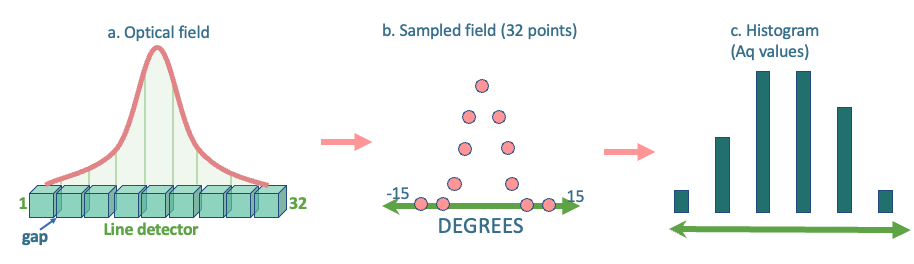
\includegraphics{notebooks/figures/a/fig_1_optical_field.png}

}

\caption{\label{fig-2-1}a. Optical field definition. b. Window
integration. c.~Histogram}

\end{figure}

\hypertarget{optical-field-and-window-integration-simulation}{%
\section{Optical field and window integration
simulation}\label{optical-field-and-window-integration-simulation}}

The optosurf signal is reconstructed from the 32 sampling points. Such
sampling points characterize the roughness of any given sample through
the parameters \(\mu\) and \(\sigma\). The \(\mu\) parameter relates to
the incoming angle of the sample's reflected light, this is equivalent
to a lateral shift of the optical field. The \(\sigma\) parameter
relates roughness of the sample and determines the width of the optical
field.

This is shown in Figure~\ref{fig-2-2}. When a wafer is rotated the
optosurf signal is displaced along the linear detector, while increasing
the sample roughness widens the optosurf signal through the \(\sigma\)
parameter.

\begin{figure}

{\centering 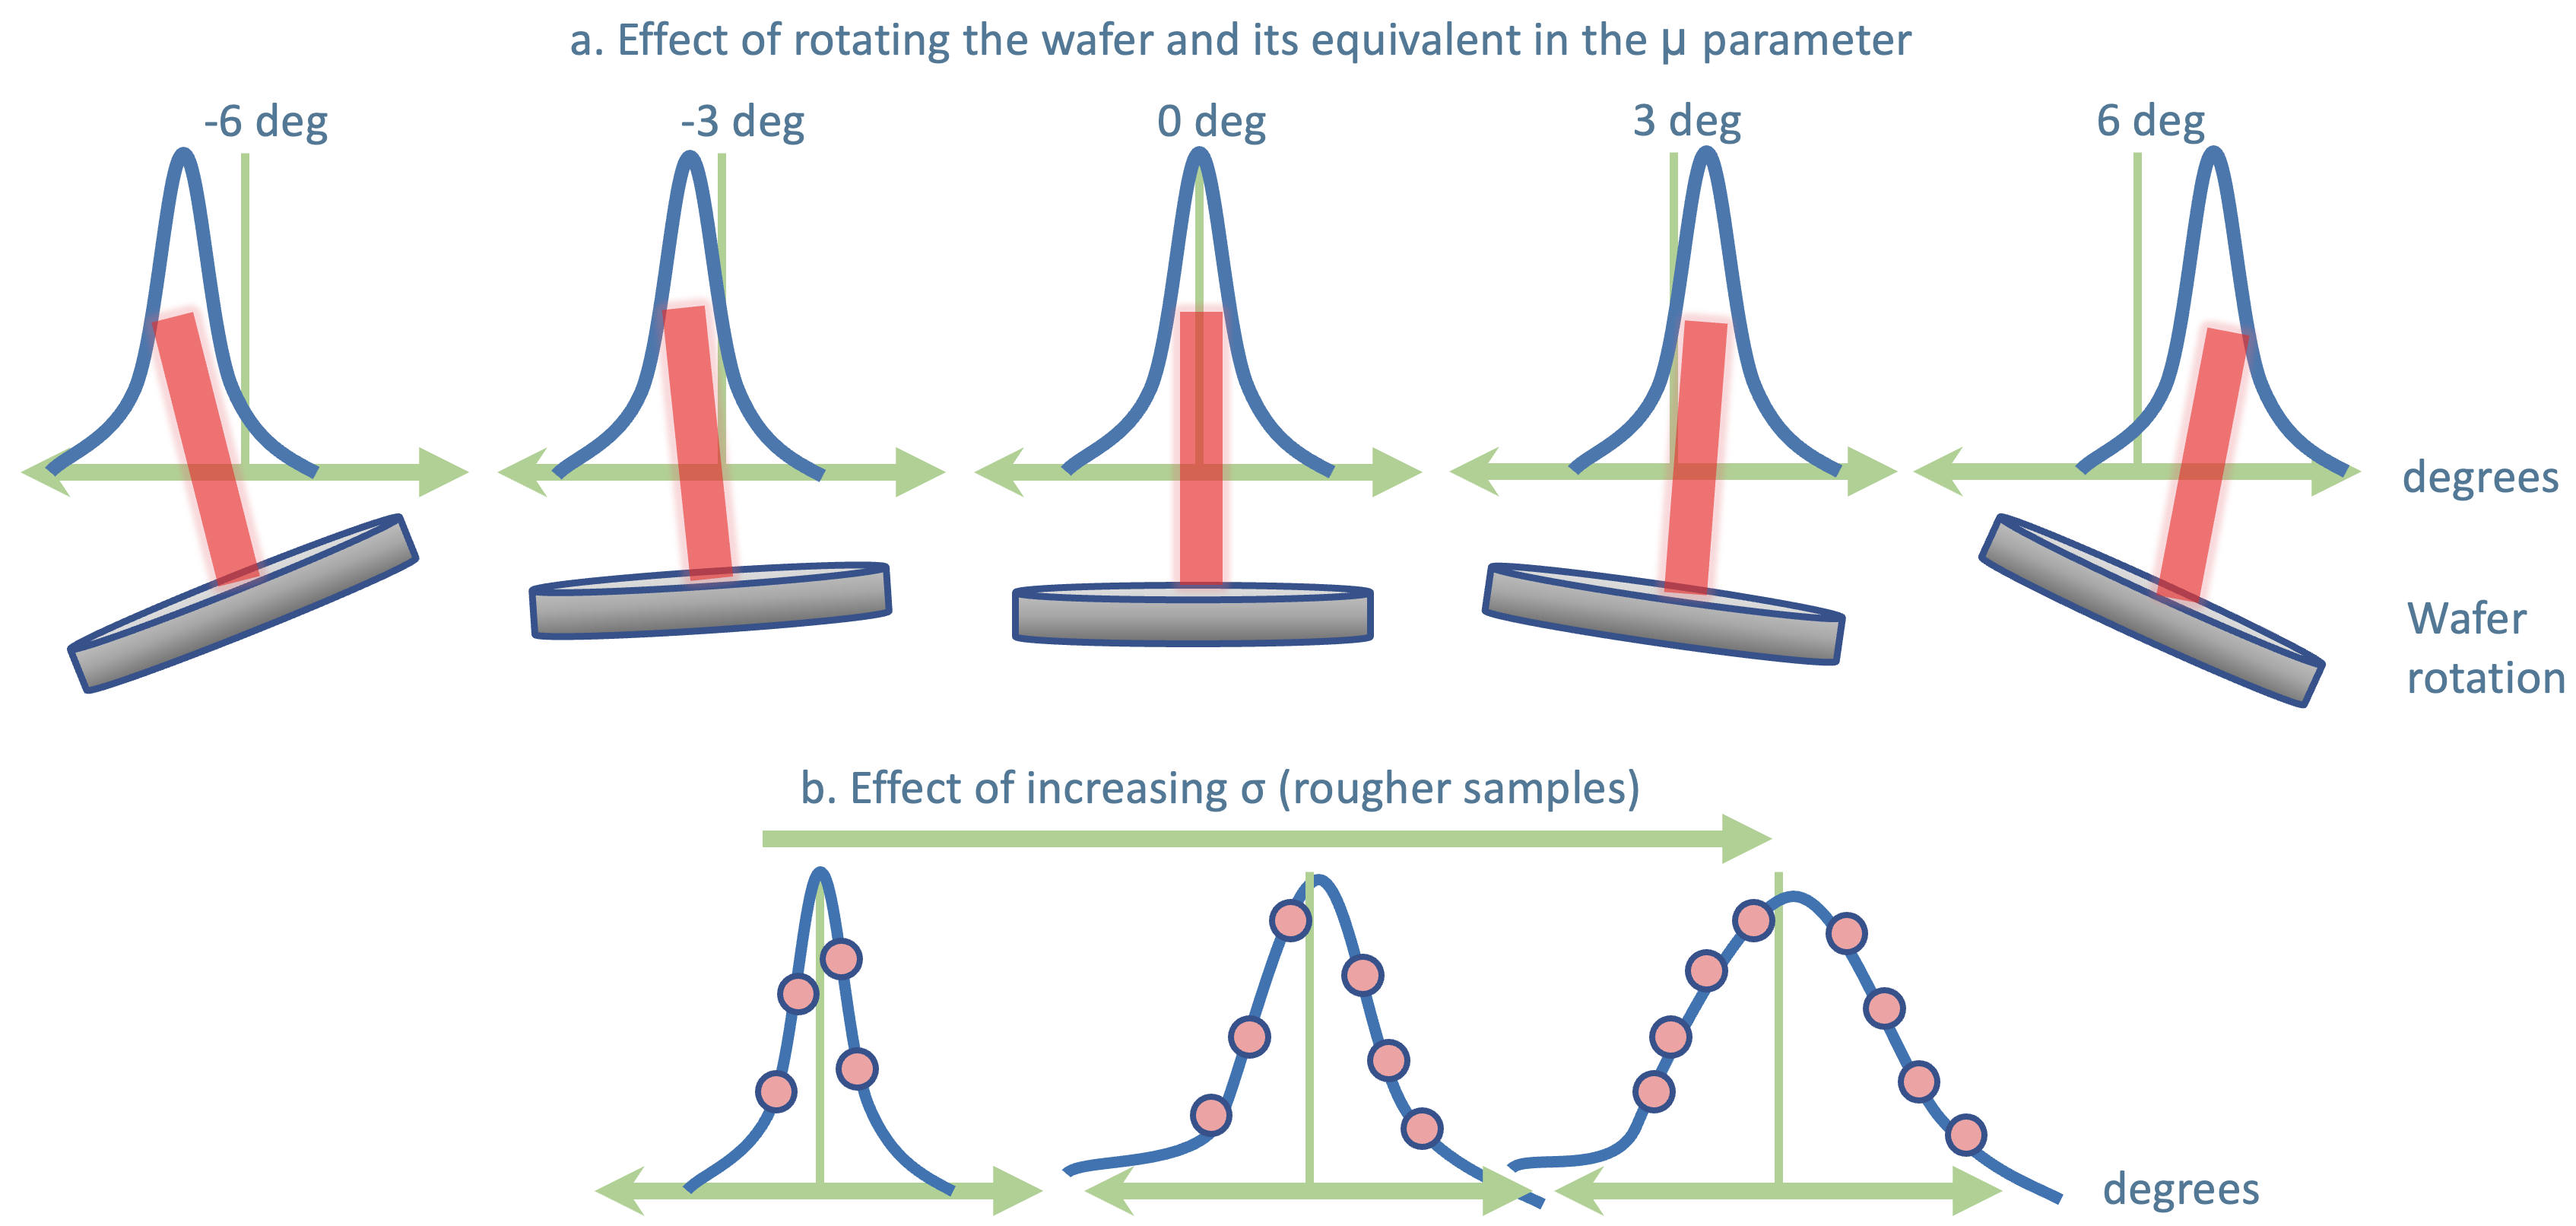
\includegraphics{notebooks/figures/a/fig_2_wafer_rotation.png}

}

\caption{\label{fig-2-2}a. Effect of changing the angle of the incoming
light. b. Effect of increasing sample roughness}

\end{figure}

In order to simulate this, the equation of an optical field is defined
as:

\(y = e^{-((x-\mu)/\sigma)^n}\)

Then, different parameters for \(\mu\) and \(\sigma\) are used to
simulate different optical fields over a range of 30 degrees from -15 to
15, as shown in Figure~\ref{fig-2-3-histogram} (a). Notice when changing
\(\mu\) from -4.0 to 4.0 the optical field is displaced along the linear
detector. When changing \(\sigma\) from 1.0 to 2.5 the optical field is
widened.

In order to simulate the linear array detector, a window integration was
performed over the optical field representing each pixel. This is
represented by the green rectangles in Figure~\ref{fig-2-3-histogram}.
Notice how for optical field with narrower peaks there are fewer
sampling points (green points), while for wider peaks there are more
sampling points. This directly relates to the Aq parameter that is
calculated from the histogram of the sampling points as shown in
Figure~\ref{fig-2-3-histogram} b.

For the case of very smooth wafer the type of signal that is expected is
a very narrow signal (small \(\sigma\)), hence the Aq parameter will be
limited to only a few sampling points along the main peak and across the
tails of the signal.

\begin{figure}

{\centering 

\begin{figure}

{\centering 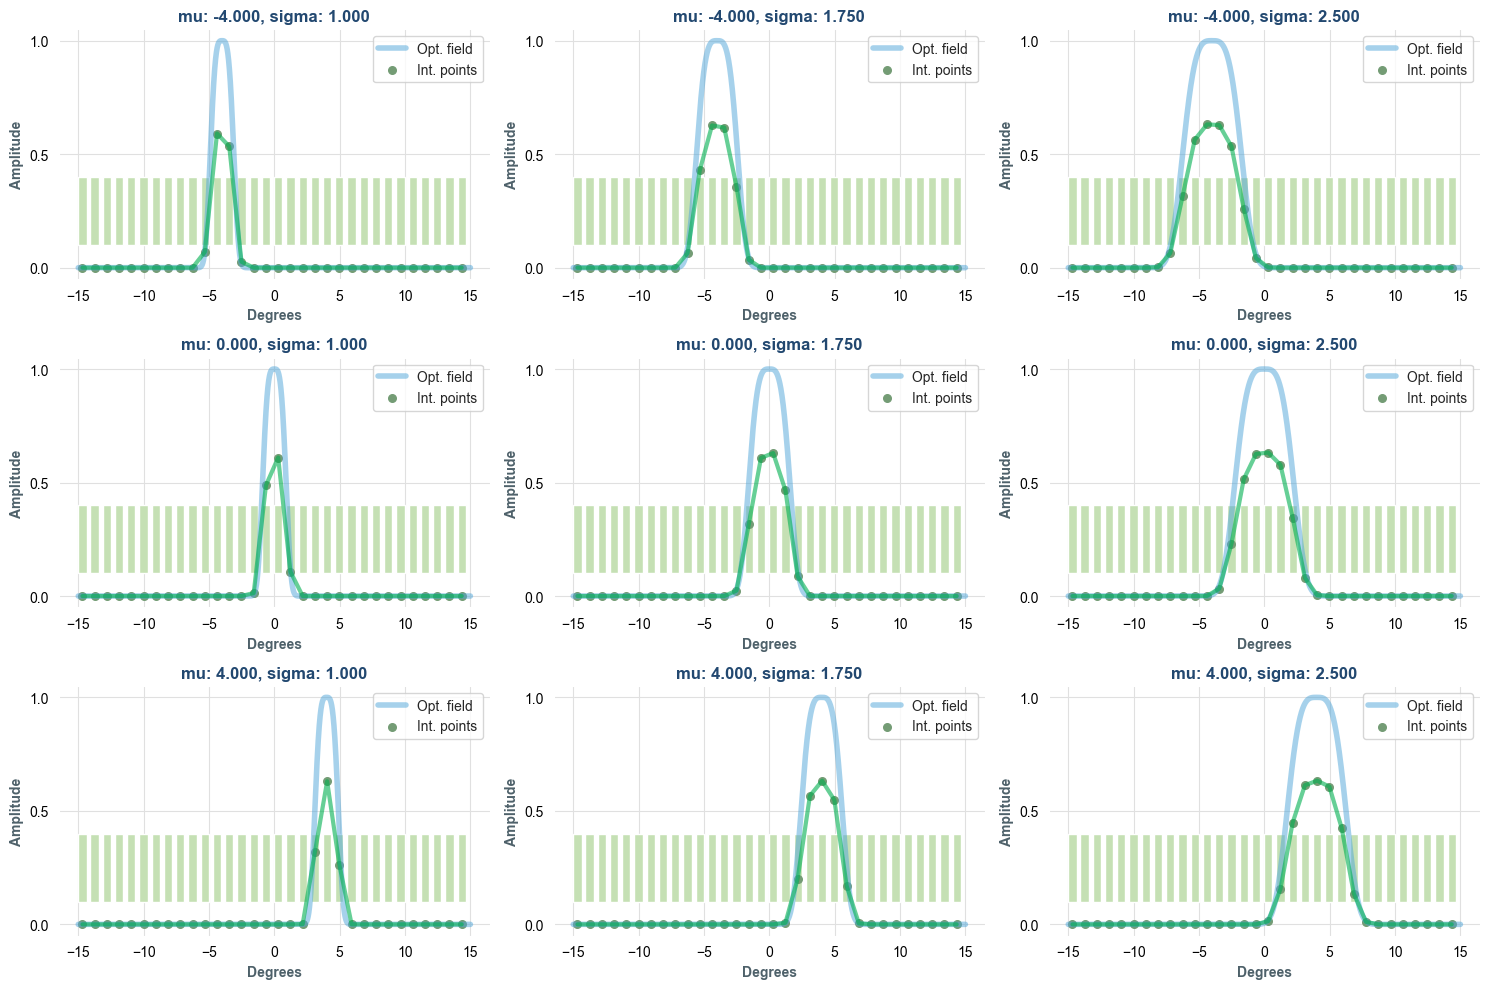
\includegraphics{notebooks/a_optical_field_files/figure-pdf/fig-2-3-histogram-output-1.png}

}

\caption{Optical field window sampling}

\end{figure}

\begin{figure}

{\centering 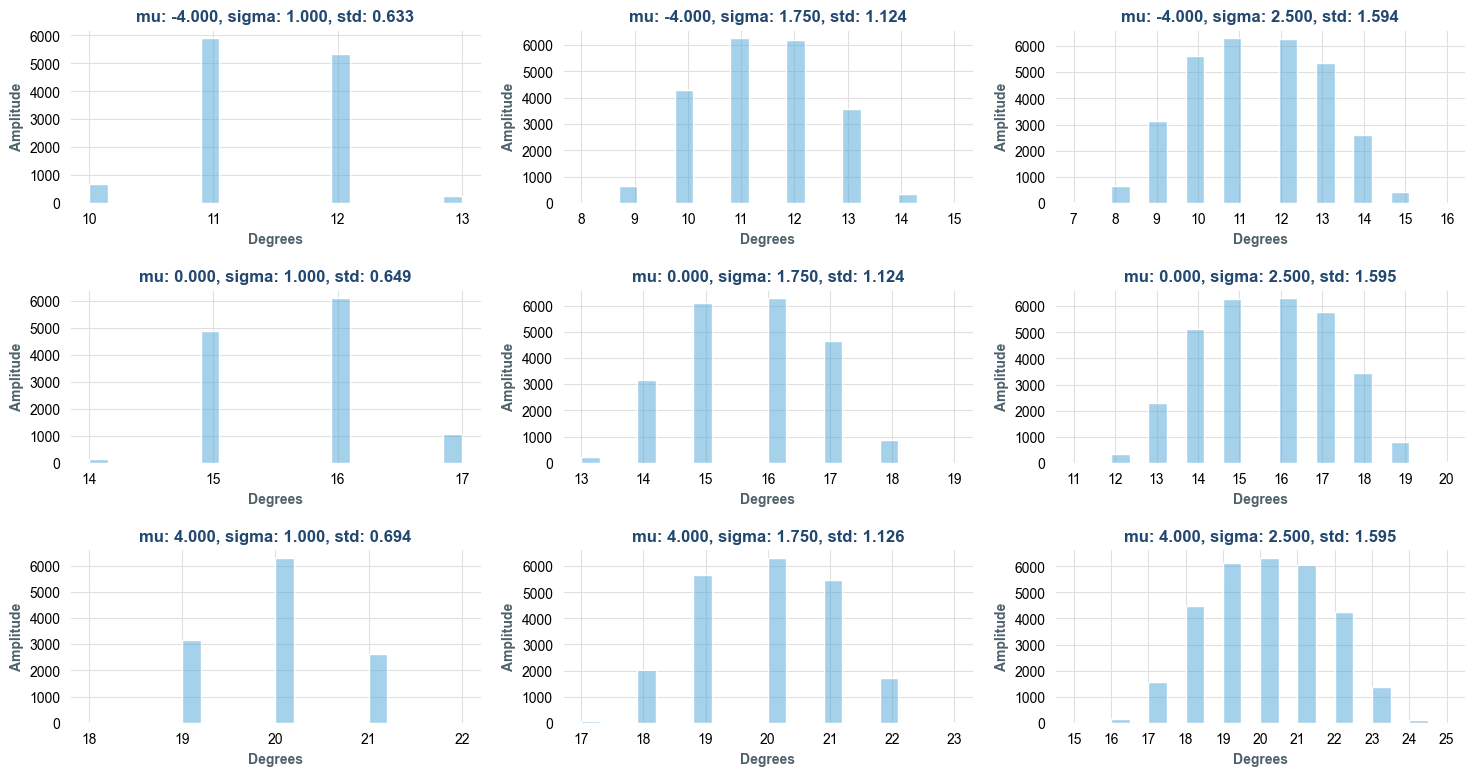
\includegraphics{notebooks/a_optical_field_files/figure-pdf/fig-2-3-histogram-output-2.png}

}

\caption{Aq histogram reconstruction}

\end{figure}

}

\caption{\label{fig-2-3-histogram}Window sampling and Aq histogram
reconstruction for different optical fields.}

\end{figure}

\hypertarget{aq-parameter-limitations}{%
\section{Aq parameter limitations}\label{aq-parameter-limitations}}

From the simulation of the linear array, it was learnt that the Aq
parameter depends on the width of the optical field. In the case of a
smooth wafer, the optical field is very narrow and the Aq parameter is
limited to only a few sampling points. Additionaly, the Aq parameter is
dependent on the incoming angle of the sample's reflected light, hence
being angle sensitive. This is illustrated in Figure~\ref{fig-2-4}:

\begin{figure*}

{\centering 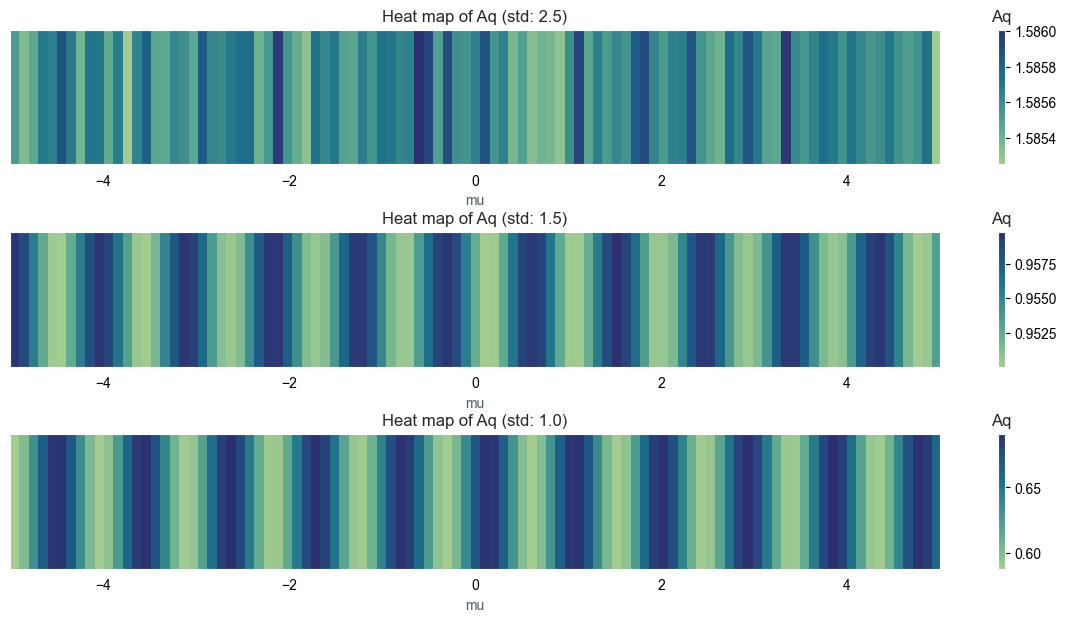
\includegraphics{notebooks/a_optical_field_files/figure-pdf/fig-2-4-output-1.png}

}

\caption{\label{fig-2-4}Aq values as function of mu and standard
deviation}

\end{figure*}

From the previous figure the Aq has the following limitations:

\begin{itemize}
\tightlist
\item
  The variation of Aq parameter is small for wider optical fields
  (larger \(\sigma\)).
\item
  In contrast, the variation of Aq parameter increases for narrower
  optical fields (smaller \(\sigma\)).
\item
  The Aq parameter is angle sensitive, specially for optical fields with
  narrower peaks (smaller \(\sigma\)).
\end{itemize}

Because of this limitations the Aq parameter would be able to
distinguish between samples with very different roughness, but it would
not be able to distinguish between samples with similar roughness,
specially with a nm roughness variation.

\newpage

\bookmarksetup{startatroot}

\hypertarget{base-function}{%
\chapter{Base function}\label{base-function}}

The sampled optical field on the line detector was previously simulated,
the observations were:

\begin{enumerate}
\def\labelenumi{\arabic{enumi}.}
\item
  There are 32 sampling points as the line detector has the same number
  of pixels. This was simulated using a window integration over a
  defined optical field defined by: \(y = e^{-((x-\mu)/\sigma)^n}\).
\item
  The parameters \(\mu\) and \(\sigma\) determine the lateral shift and
  width of the gaussian function respectively. These parameters are
  related to the incoming light angle from the sample and the material
  roughness.
\item
  The \(\mu\) parameter was swept to simulate different incoming light
  angles. With this data, a histogram was then reconstructed and its
  standard deviation value was calculated.
\item
  An oscillating pattern was observed in the histogram's standard
  deviation (Aq parameter). This is not ideal as this indicated a
  roughness change, however only the angle of the incoming light was
  being swept.
\item
  Hence, a new parameter that is constant as a function of \(\mu\) has
  to be found.
\end{enumerate}

In order to obtain such new parameter a base function is proposed as
shown in Figure~\ref{fig-3-1} :

\begin{figure}

{\centering 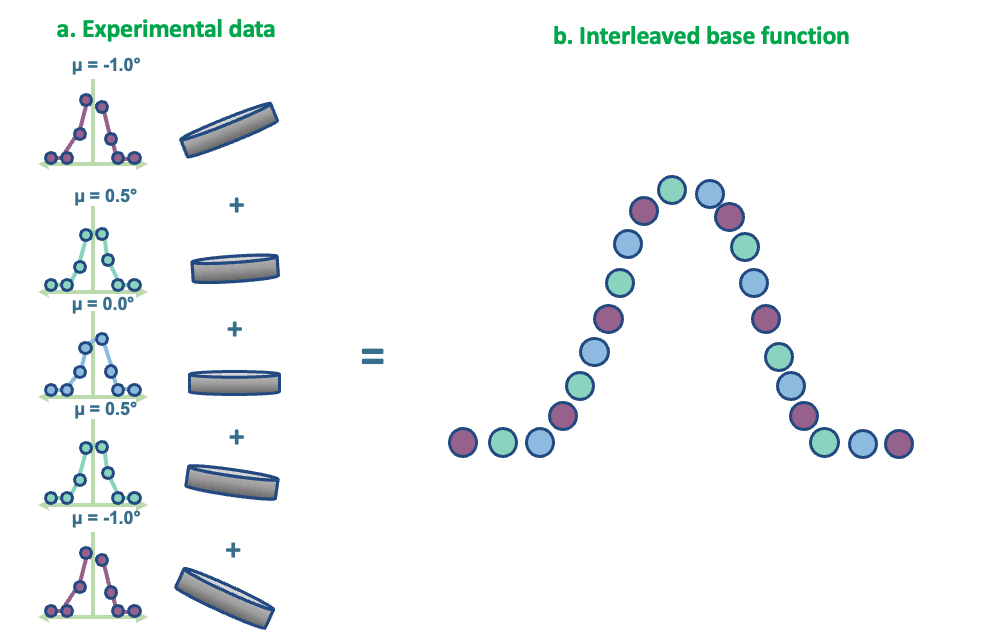
\includegraphics{notebooks/figures/b/fig_3_1_base.png}

}

\caption{\label{fig-3-1}a. Experimental data acquired at different
incoming angles. b. Base function reconstruction}

\end{figure}

The idea of the base function consists in reconstructing a reference
function obtained from experimental data of a very smooth wafer (0.1 nm
in roughness) at different angles in order to obtain a function that is
constant as a function of \(\mu\). This function will then be used as a
reference parameter to compare with the experimental data of rougher
wafers (1 nm). The reconstruction of the base function is illustrated in
the previous image.

\hypertarget{base-function-simulation}{%
\section{Base function simulation}\label{base-function-simulation}}

The mathematical procedure for the base function reconstruction consists
in sampling the optical fields at different incoming angles and the
reshifting such points to the 0 deg reference, obtaining a higher
density of sampling points instead of the limited 32 sampling points.
This is shown in Figure~\ref{fig-3-2} and Figure~\ref{fig-3-3} (higher
density of sampling points).

\begin{figure}

{\centering 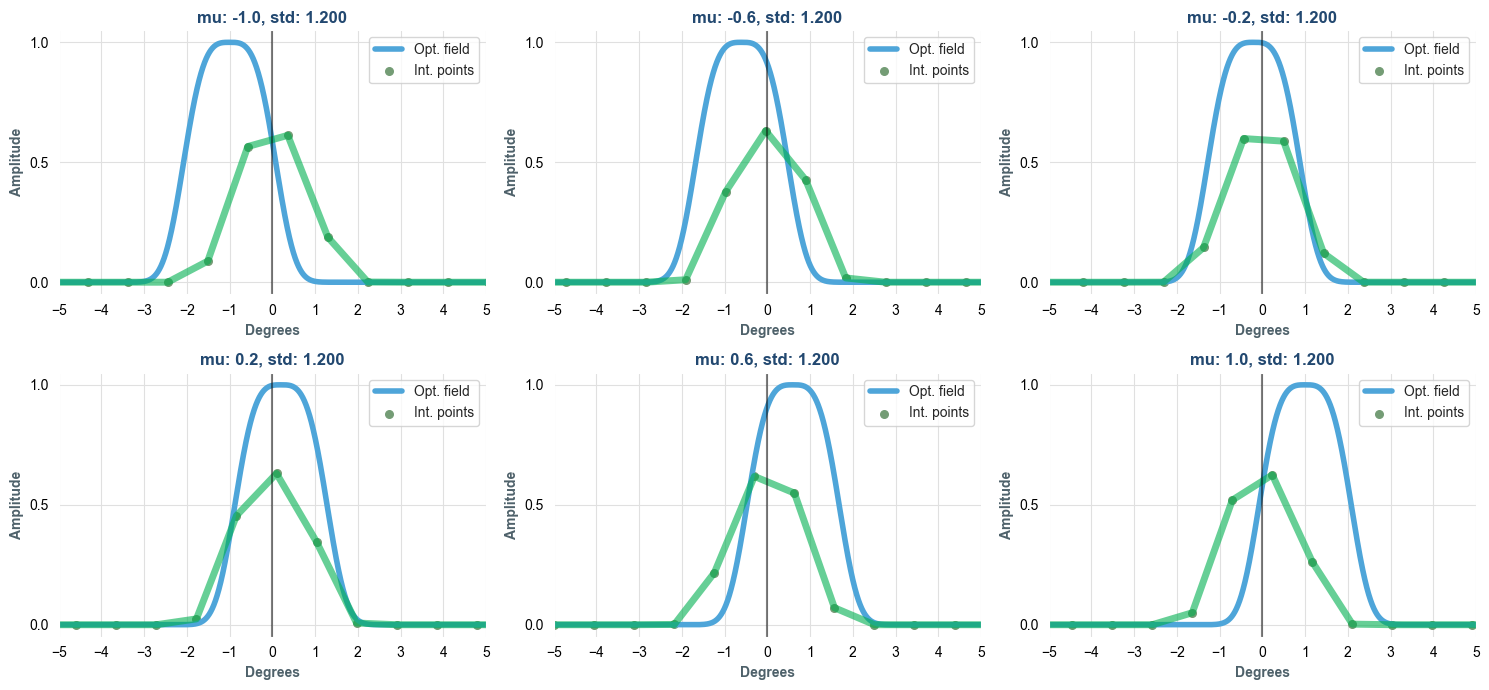
\includegraphics{notebooks/b_base_function_files/figure-pdf/fig-3-2-output-1.png}

}

\caption{\label{fig-3-2}Reconstruction of base function from shifted
optical fields}

\end{figure}

\begin{figure}

{\centering 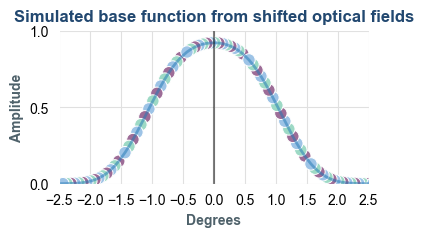
\includegraphics{notebooks/b_base_function_files/figure-pdf/fig-3-3-output-1.png}

}

\caption{\label{fig-3-3}Base function with higher density of sampling
points}

\end{figure}

\hypertarget{test}{%
\section{Experimental base function}\label{test}}

The base function is meant to be a reference function in order to
characterize wafer roughness. For such purpose, a very smooth wafer (0.1
nm in roughness) was measured at different angles. The base function was
then reconstructed using the same procedure as the simulated base
function. The experimental data is shown in Figure~\ref{fig-3-4}. The
collected angles were from -1.0 to 1.0 degrees.

\begin{figure}

{\centering 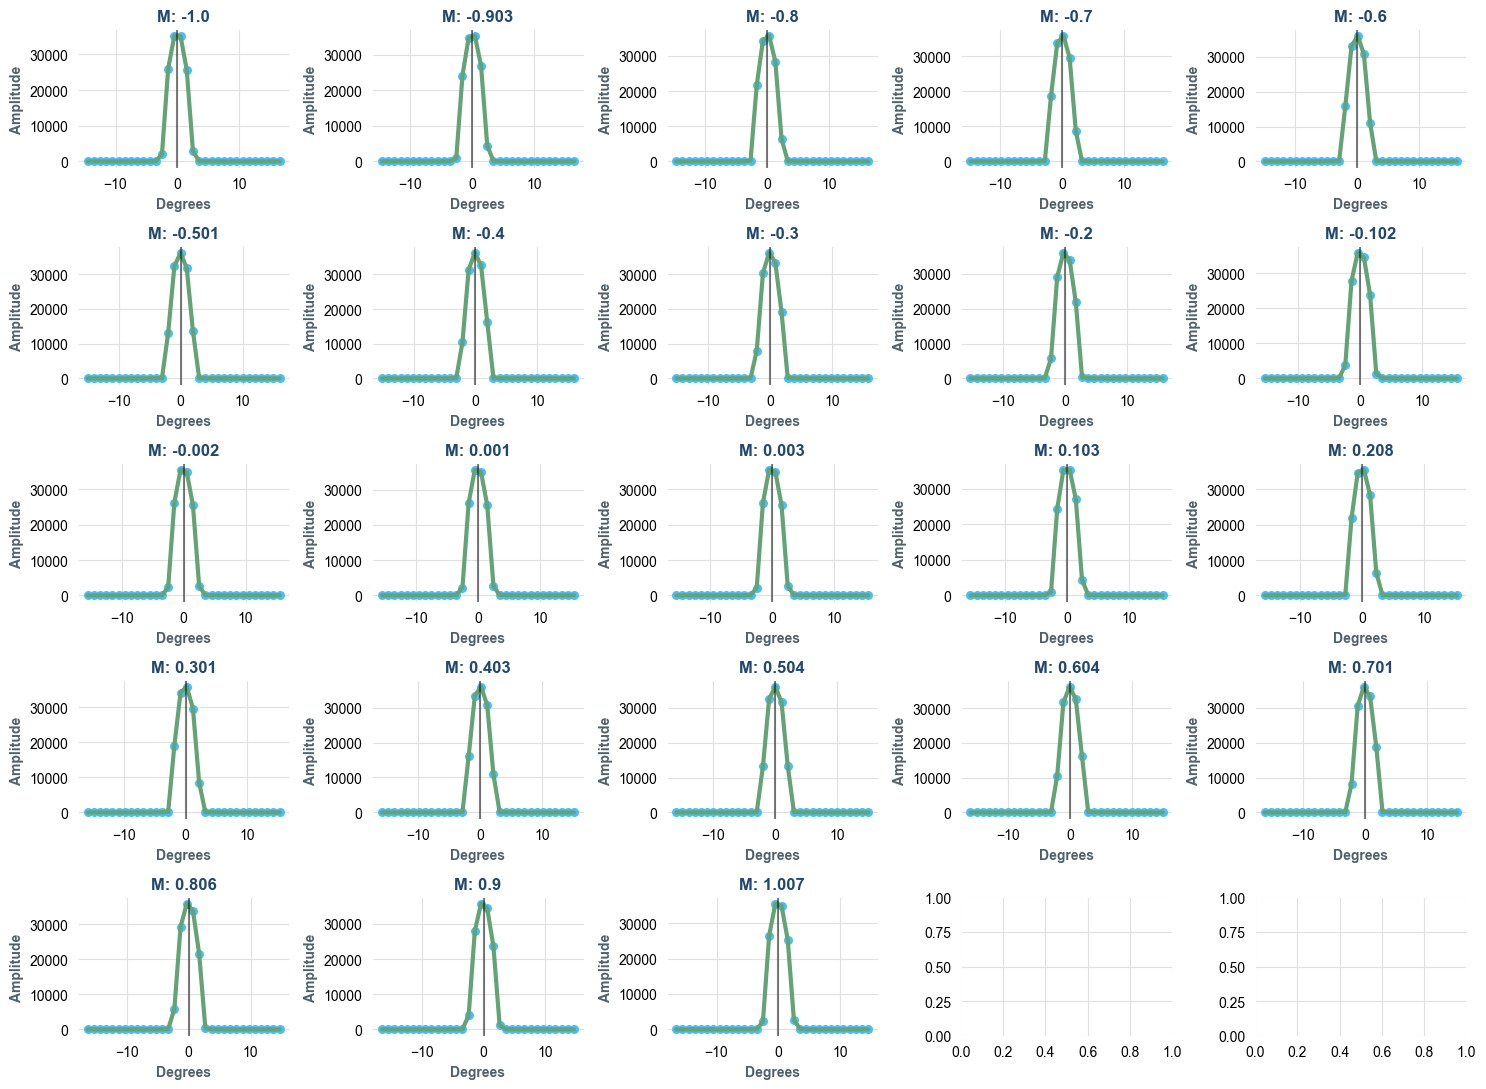
\includegraphics{notebooks/b_base_function_files/figure-pdf/fig-3-4-output-1.png}

}

\caption{\label{fig-3-4}Smooth wafer experimental data for base function
reconstruction}

\end{figure}

The procedure from the simulated base function was then applied to the
experimental data. The results are shown in Figure~\ref{fig-3-5}. Notice
that there are some overlaps in the sampling points, this is due to
innacurate angle measurements. However, this base function can be use as
a reference for further data correction.

One of the main difference between using just the Aq parameter compared
to the base function is the number of sampling for very smooth wafers.
The base function has a higher density of points in the tails as well as
in the main peak.

\begin{figure}

{\centering 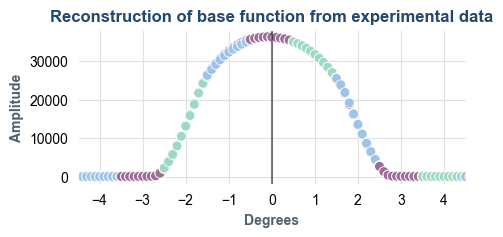
\includegraphics{notebooks/b_base_function_files/figure-pdf/fig-3-5-output-1.png}

}

\caption{\label{fig-3-5}Reconstructed base function from experimental
data}

\end{figure}

\hypertarget{on-axis-and-off-axis-datasets}{%
\section{On-axis and off-axis
datasets}\label{on-axis-and-off-axis-datasets}}

One of the limitations of the previous data, was that the exact incoming
angle was not known, hence there was overlap in the sampling points. To
compensate for this, a setup was built and shown in Figure~\ref{fig-3-6}
:

\begin{figure}

{\centering 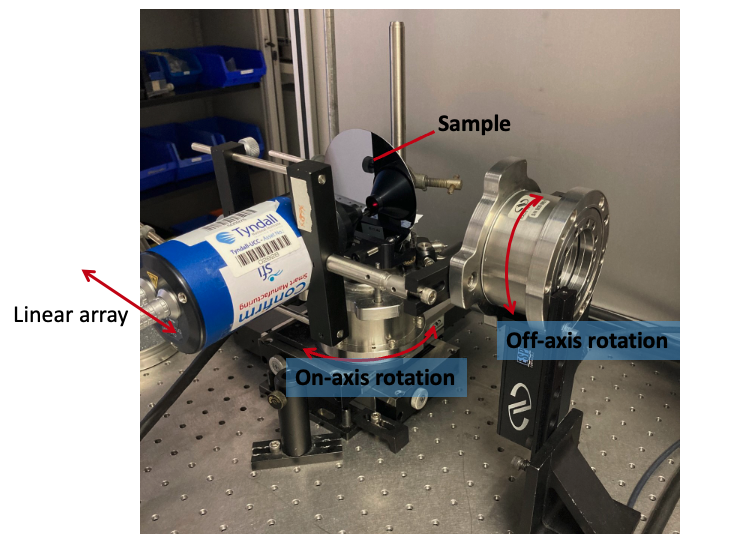
\includegraphics{notebooks/figures/b/fig_3_2_setup.png}

}

\caption{\label{fig-3-6}OS500 head is attached to off-axis motor, and
points at centre of rotation. Sample is attached to on-axis motor, and
positioned at centre of rotation. Additionally there are two linear
stages for positioning. All motors are PC controlled}

\end{figure}

With this setup it is possible to acquire datasets along the optosurf
axis (on-axis) at different vertical off-axis misalignment positions.
Both axes are illustrated in Figure~\ref{fig-3-7} :

\begin{figure}

{\centering 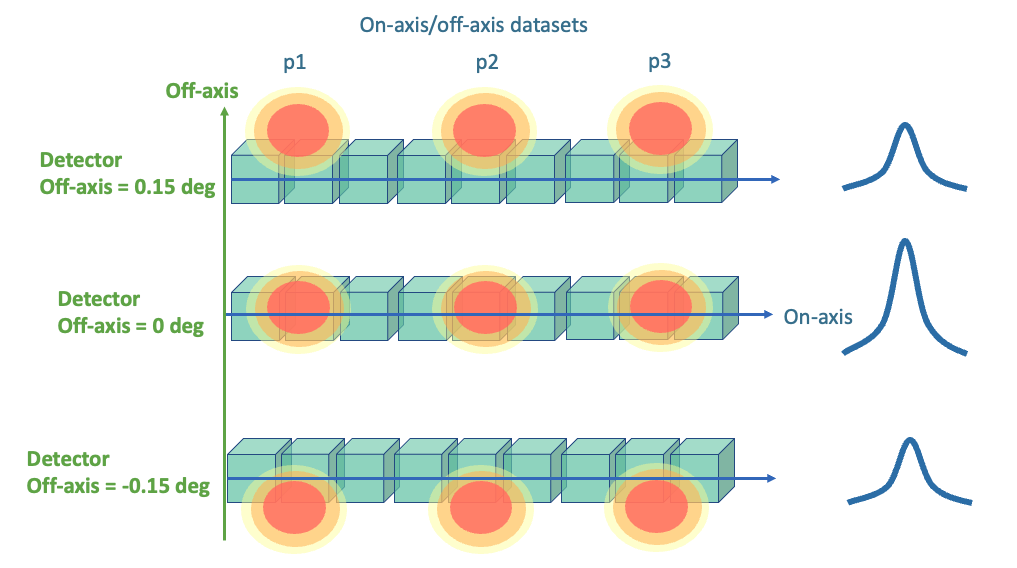
\includegraphics{notebooks/figures/b/fig_3_3_onoffaxis.png}

}

\caption{\label{fig-3-7}On-axis datasets at off-axis positions. Data is
collected along the on-axis position with scanning angles of 20 deg. The
same dataset is collected at different off-axis positions for example at
+- 0.15 deg. Notice that the amplitude decreases for off-axis
positions.}

\end{figure}

One of the reasons for acquiring the dataset in both on-axis and
off-axis positions is due to the very narrow peak obtained from the
scattered light of the Si wafer. The idea is to acquire a dataset along
the on-axis at 4000 angle positions (each position has a 32 points data
trace) within +-20 deg, and at different off-axis positions for example
between +- 0.15 deg. With these datasets it will be posible to
reconstruct a base function at different off-axis positions and obtain
the angles at which the new RMSE parameter will be valid for.

An example of a on-axis dataset is shown in Figure~\ref{fig-3-8}.
Different traces are also shown for different positions along the
mechanical axis. It is with the on-axis dataset that the base function
will be reconstructed.

\begin{figure}

{\centering 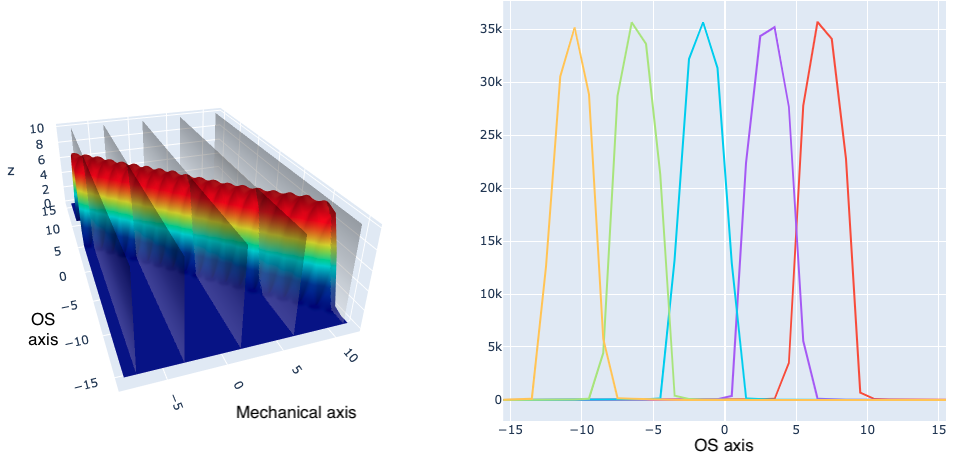
\includegraphics{notebooks/figures/b/fig_3_3_onaxis.png}

}

\caption{\label{fig-3-8}On-axis dataset. The gray planes are
cross-sections that represent that 32 sampling points optosurf traces}

\end{figure}

The off-axis data is taken along the perpendicular axis of the linear
array. When the head is aligned at the center the intensity of the
optical field will be maximum. As the mechanical axis scans, the
amplitude will start decreasing due to the `off-axis' alignment. The
dataset is shown in Figure~\ref{fig-3-9}.

\begin{figure}

{\centering 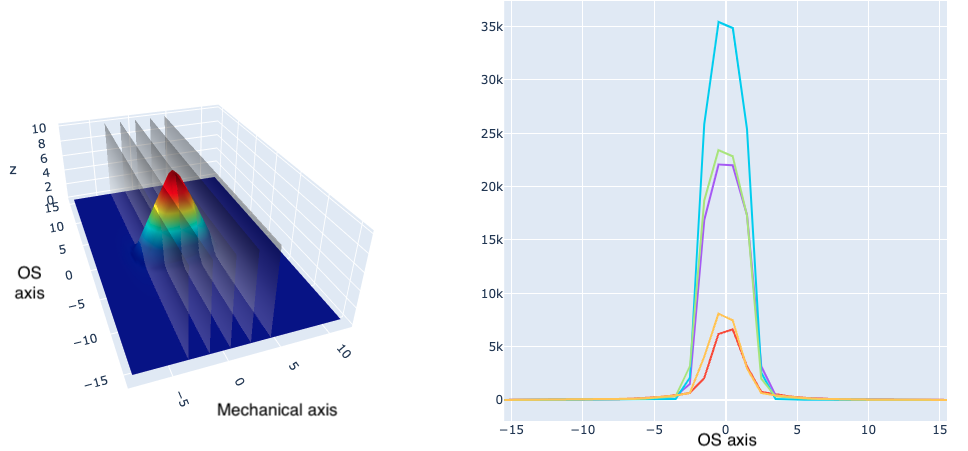
\includegraphics{notebooks/figures/b/fig_3_4_offaxis.png}

}

\caption{\label{fig-3-9}On-axis dataset. The gray planes are
cross-sections that represent that 32 sampling points optosurf traces}

\end{figure}

\newpage

\bookmarksetup{startatroot}

\hypertarget{minimization-methods}{%
\chapter{Minimization methods}\label{minimization-methods}}

The setup shown in Figure~\ref{fig-3-6} was used to obtain on-axis data
to reconstruct base functions at different off-axis position. The
methodology for this is described in Figure~\ref{fig-4-1} :

\begin{figure}

{\centering 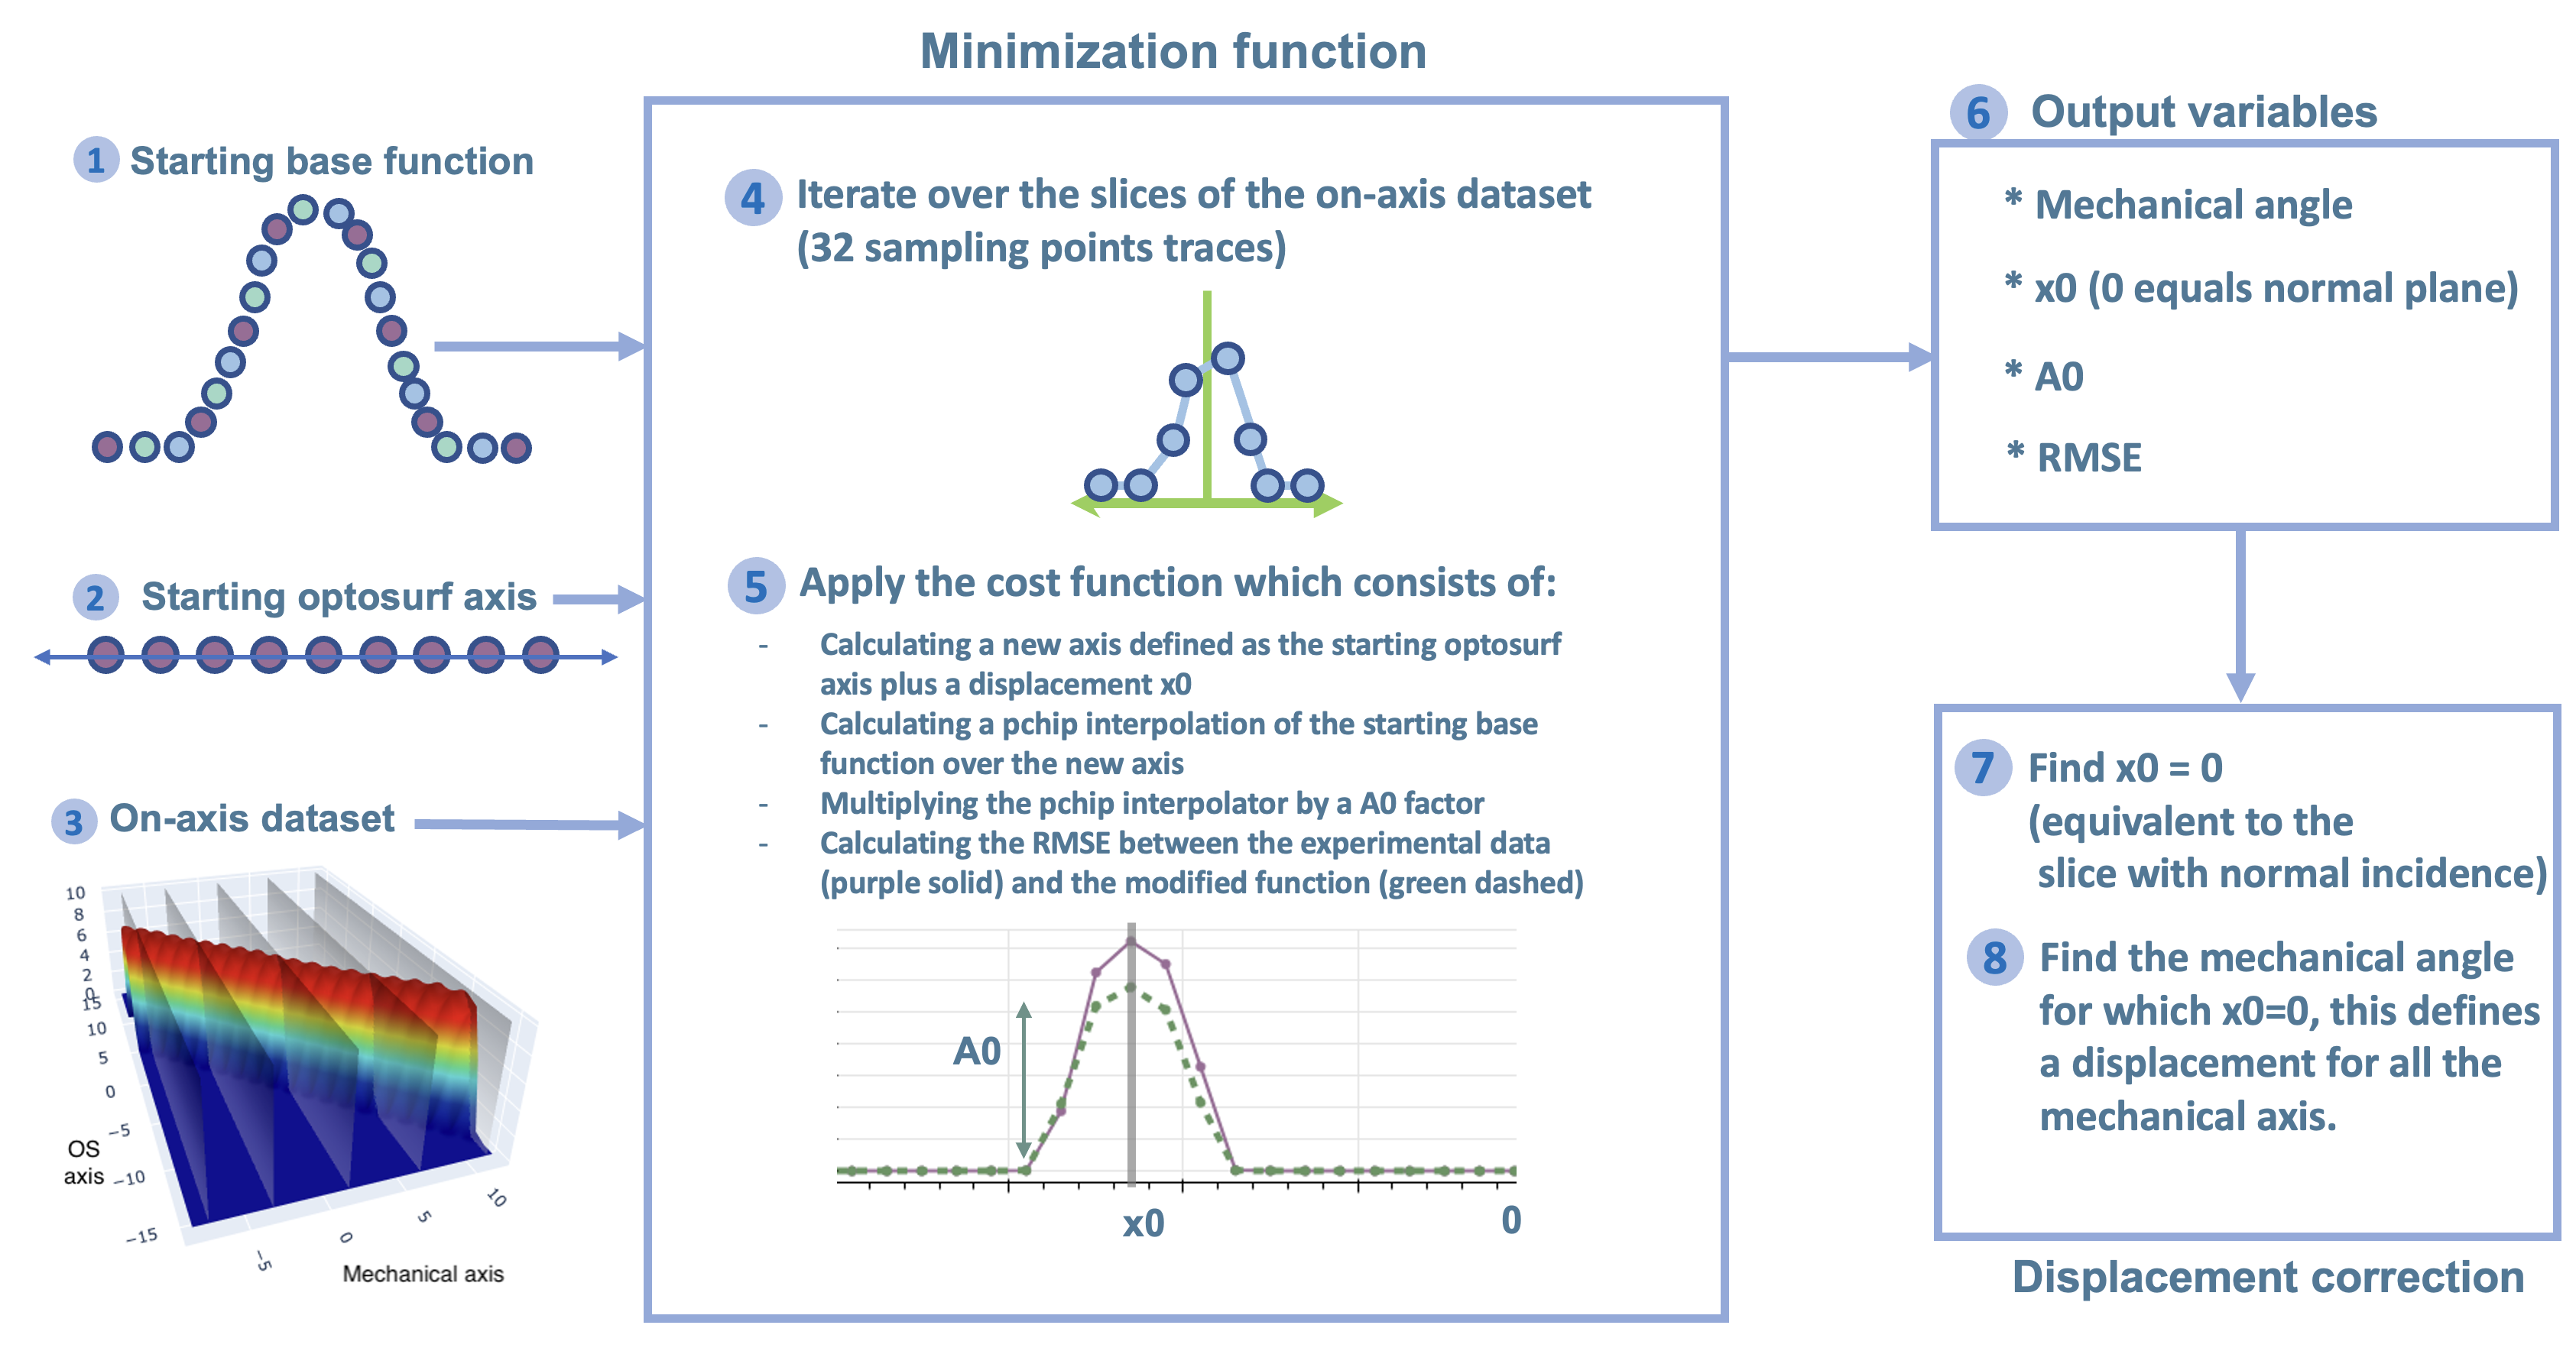
\includegraphics{notebooks/figures/c/fig_4_1_minimization.png}

}

\caption{\label{fig-4-1}Methodology to acquire a base function}

\end{figure}

\begin{enumerate}
\def\labelenumi{\arabic{enumi}.}
\item
  \textbf{Starting base function:} The reconstructed base function from
  Figure~\ref{fig-3-5} was used as a starting function even if the
  sampling points were not perfectly aligned with their corresponding
  angles.
\item
  \textbf{Starting optosurf axis:} These are the 32 pixels that go from
  -15 to 15 deg with 1 deg steps.
\item
  \textbf{On-axis dataset:} An on-axis dataset of very Si smooth wafers
  (0.1 nm roughness). The mechanical axis was acquired within an angle
  range with a certain numbers of slices, for example +-20 deg
  (equivalent to 40 deg due to reflection angle) with 4096 slices. Each
  slice has a 32 sampling points optosurf trace.
\end{enumerate}

\textbf{Minimization function:}

\begin{enumerate}
\def\labelenumi{\arabic{enumi}.}
\setcounter{enumi}{3}
\item
  \textbf{Iteration over the slices of the on-axis dataset:} Each slice
  of the on-axis dataset is iterated and is used as the reference
  experimental data to be fit.
\item
  \textbf{Applying cost/minimization function:} This function takes the
  experimental data and makes a fit using three parameters:
\end{enumerate}

\begin{itemize}
\tightlist
\item
  x0 - Equivalent to a lateral displacement of the base function.
\item
  A0 - A factor multiplying the amplitude of the base function.
\item
  pchip interpolator - A pchip (Piecewise Cubic Hermite Interpolating
  Polynomial) interpolator is an algorithm used to smooth the base
  function to a 32 points xaxis (starting optosurf axis + x0).
\end{itemize}

\begin{enumerate}
\def\labelenumi{\arabic{enumi}.}
\setcounter{enumi}{5}
\tightlist
\item
  \textbf{Output variables:} The output variables of the minimization
  function are:
\end{enumerate}

\begin{itemize}
\tightlist
\item
  The mechanical angle (corresponding to the mechanical scanning)
\item
  x0 - Equivalent to a lateral displacement of the base function. Notice
  that x0 = 0 is the reference to know where the light is normally
  incident to the optosurf head.
\item
  A0 - A factor multiplying the amplitude of the base function.
\item
  RMSE - The optimization error measurement
\end{itemize}

\textbf{Displacement correction}

\begin{enumerate}
\def\labelenumi{\arabic{enumi}.}
\setcounter{enumi}{6}
\item
  \textbf{Find x0 = 0 (normal incident plane)}
\item
  \textbf{Find the mechanical angle corresponding to x0 = 0:} This
  defines a displacement correction angle for the mechanical axis such
  that zero degrees correspond to the x0 of the optosurf axis.
\end{enumerate}

\hypertarget{datasets}{%
\section{Datasets}\label{datasets}}

The acquired on-axis and off-axis datasets are shown in
Figure~\ref{fig-4-2} :

\begin{figure}

{\centering 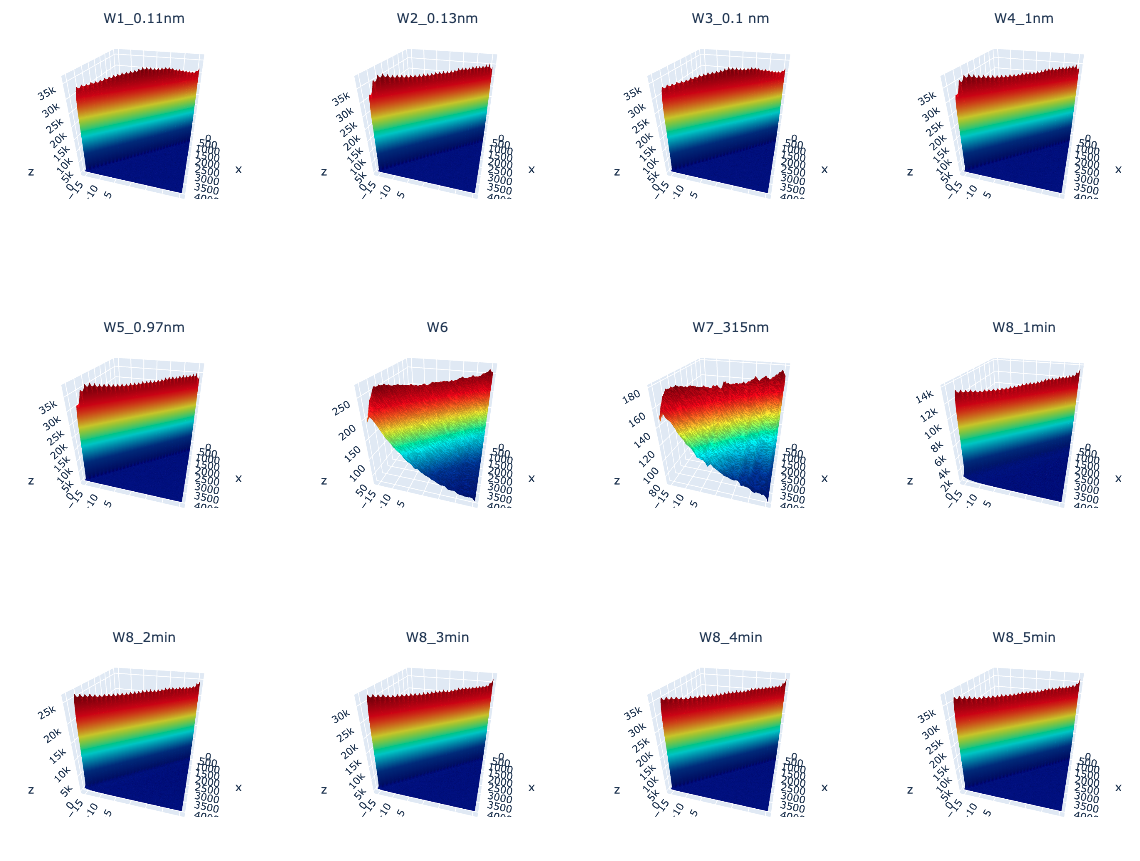
\includegraphics{notebooks/figures/c/fig_4_2_datasets.png}

}

\caption{\label{fig-4-2}On-axis datasets. Notice that as the roughness
increases the amplitude decreases as well as becoming broader}

\end{figure}

These datasets were acquired along the on-axis within an angle of 20 deg
(40 deg due to double reflection angle) and at 6 different off-axis
positions from -0.150 to 0.150 deg in 0.05 deg steps. Notice how for
much smoother wafers (0.1 nm) the signal amplitude is much higher
(around 35,000 in amplitude). As the sample becomes rougher the
amplitude decreases and the signal becomes wider as well. This is
illustrated in the Ann 1 min - Ann 5 min. The time represents the polish
time, as the sample becomes smoother with higher polishing time the
amplitude increases.

The parameters for each dataset are shown in Table~\ref{tbl-1}. The
datasets with a roughness of 0.1 nm are used as the reference to
reconstruct the base function. The RMSE is then calculated with respect
to these base functions for rougher wafers.

\hypertarget{tbl-1}{}
\begin{longtable}[]{@{}llll@{}}
\caption{\label{tbl-1}On-axis and off-axis datasets
parameters}\tabularnewline
\toprule\noalign{}
& roughness (nm) & points & angle \\
file & & & \\
\midrule\noalign{}
\endfirsthead
\toprule\noalign{}
& roughness (nm) & points & angle \\
file & & & \\
\midrule\noalign{}
\endhead
\bottomrule\noalign{}
\endlastfoot
Ann10 & 0.1 & 4096 & 20 \\
PT\_ref & 0.1 & 4096 & 20 \\
Rockley\_ref & 0.1 & 4096 & 20 \\
Ann5 & 1.0 & 4096 & 20 \\
Ann7 & 1.0 & 4096 & 20 \\
PT\_3um & NaN & 4096 & 20 \\
Rockley\_rough & 1000.0 & 4096 & 20 \\
Ann\_5min & NaN & 4096 & 20 \\
Ann\_4min & NaN & 4096 & 20 \\
Ann\_3min & NaN & 4096 & 20 \\
Ann\_2min & NaN & 4096 & 20 \\
Ann\_1min & NaN & 4096 & 20 \\
\end{longtable}

\hypertarget{minimization-1st-iteration}{%
\section{Minimization 1st iteration}\label{minimization-1st-iteration}}

Once the datasets have been acquired the 1st step is to apply the
minimization function (steps 4 and 5) of Figure~\ref{fig-4-1} for each
of the 4096 slices of the dataset. The output of the minimization
function is the mechanical angle, x0, A0 and RMSE. The normal incidence
is defined at x0 = 0, with this a displacement correction factor is
calculated for the mechanical axis (step 7 and 8 of
Figure~\ref{fig-4-1}).

The output of the minimization function for the wafers used a base
function (0.1 nm roughness) is shown in Figure~\ref{fig-4-3} :

\begin{figure}

{\centering 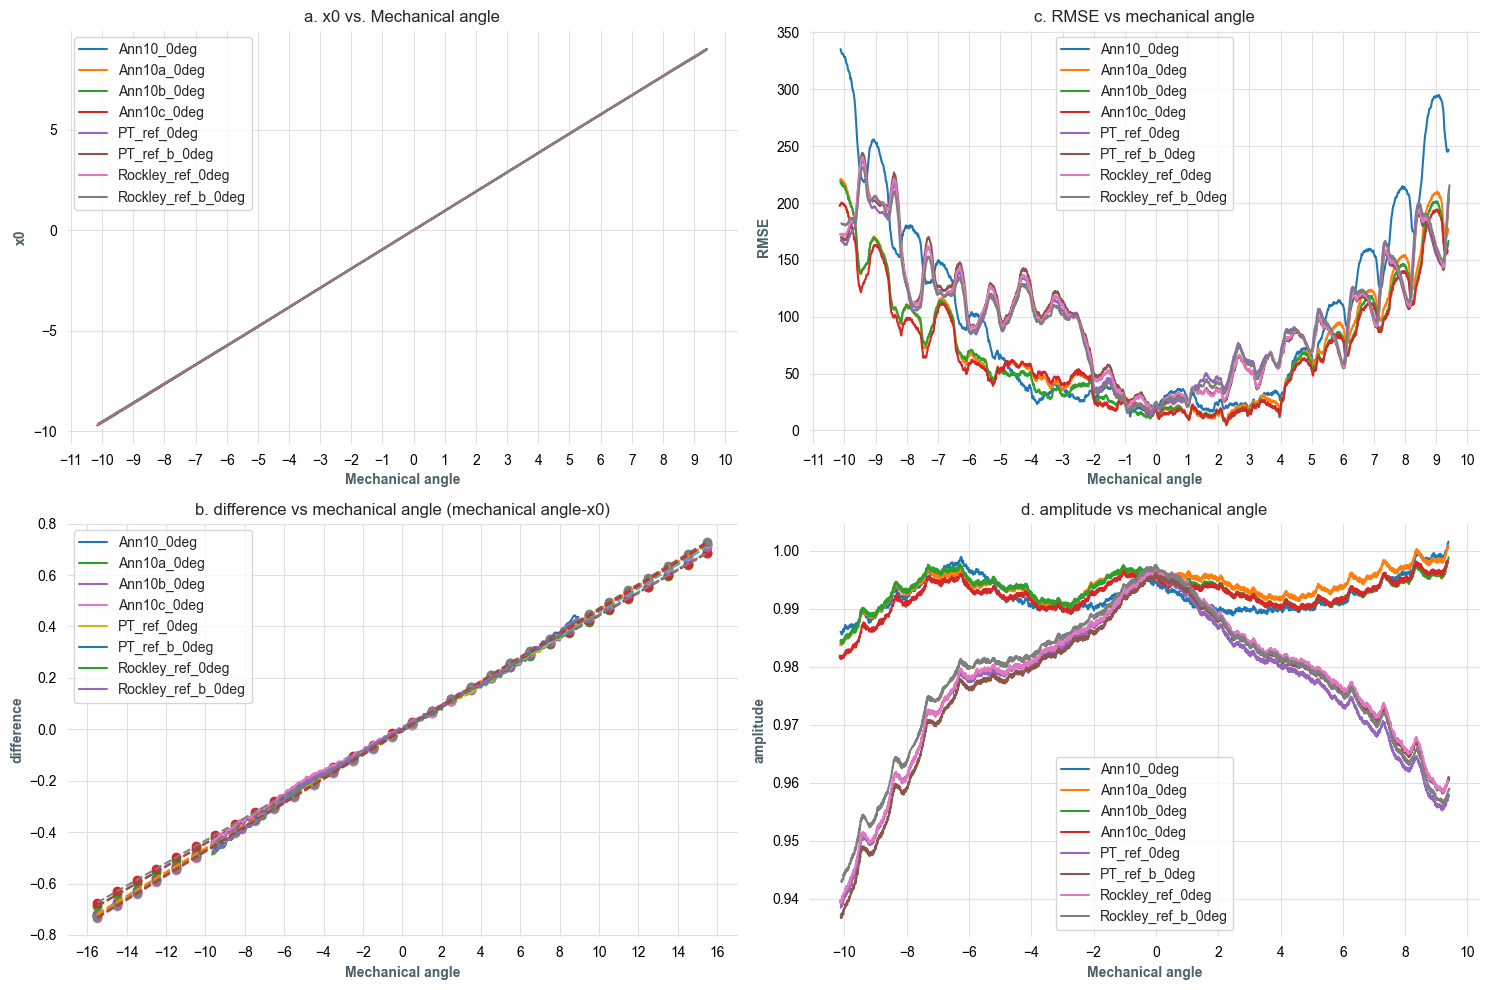
\includegraphics{notebooks/c_optimization_files/figure-pdf/fig-4-3-output-1.png}

}

\caption{\label{fig-4-3}1st optimization iteration for 0.1 nm Si wafers}

\end{figure}

The meaning of the plots is:

\begin{enumerate}
\def\labelenumi{\alph{enumi}.}
\item
  x0 vs mechanical angle. The mechanical angle is the known scanning
  angle position from the scanning along the on-axis. x0 is the fit
  parameter of the minimization function. Notice that x0 = 0 is the
  reference to know where the light is normally incident to the optosurf
  head. If they both cross at 0,0 then the mechanical axis is aligned
  with the optosurf axis. If they don't cross at 0,0 then there is a
  displacement between the mechanical axis and the optosurf axis. This
  displacement is corrected by applying a correction factor to the
  mechanical axis.
\item
  difference vs mechanical angle (mechanical angle-x0). This is the plot
  of difference between the mechanical angle and the x0. Ideally, after
  more optimization iterations the difference will converge to zero.
  With this difference a new optosurf axis is calculated.
\item
  RMSE vs mechanical angle. This plot is the RMSE per slice calculated
  from the minimization function. Ideally, after more optimization
  iterations the RMSE will converge to zero.
\item
  amplitude vs mechanical angle. This is the amplitude correction factor
  calculated from the minimization function.
\end{enumerate}

The optosurf shifted axis for the 1st iteration is shown in
Figure~\ref{fig-4-4} :

\begin{figure}

{\centering 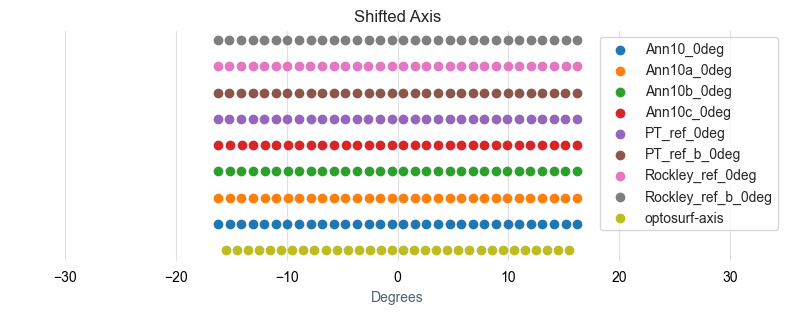
\includegraphics{notebooks/c_optimization_files/figure-pdf/fig-4-4-output-1.png}

}

\caption{\label{fig-4-4}Optosurf shifted axis}

\end{figure}

\hypertarget{base-function-1st-iteration}{%
\section{Base function 1st
iteration}\label{base-function-1st-iteration}}

Once the minimization parameters have been calculated (x0, A0) a new
shifted axis was calculated. The process to reconstruct the base
function is to take the slices from the on-axis dataset that cover a one
degree range. The data is then plot with respect to the new shifted axis
and recentered with respect to the known mechanical angle.

With this a highest density of sampling point is obtained for the base
function. An average is then calculated and finally an interpolation is
done. Examples of base functions are shown in Figure~\ref{fig-4-5} :

\begin{figure}

{\centering 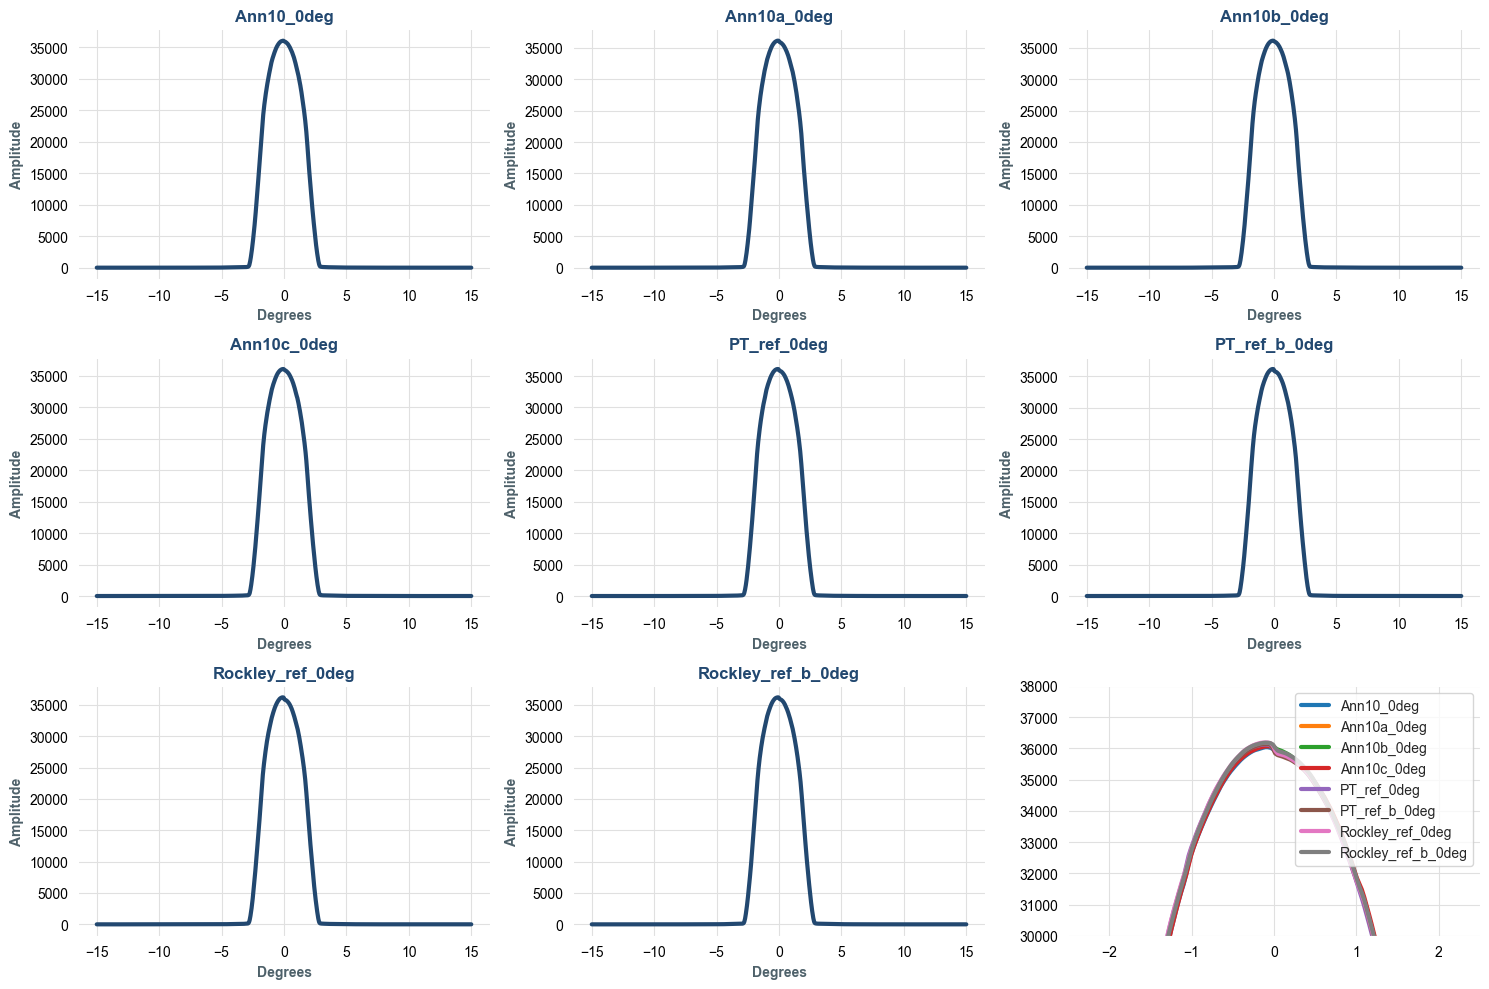
\includegraphics{notebooks/c_optimization_files/figure-pdf/fig-4-5-output-1.png}

}

\caption{\label{fig-4-5}Base functions for 0.1 nm Si wafers}

\end{figure}

\hypertarget{rmse-optimization}{%
\section{RMSE optimization}\label{rmse-optimization}}

Once the 1st iteration has been completed there are several parameters
that have been calculated:

\begin{enumerate}
\def\labelenumi{\arabic{enumi}.}
\tightlist
\item
  x0 - equivalent to the correction factor for the mechanical axis.
\item
  A0 - equivalent to the amplitude correction factor.
\item
  RMSE - the error of the minimization function.
\item
  Base function - the reconstructed base function.
\end{enumerate}

All of these variables are taken and the procedure shown in
Figure~\ref{fig-4-1} is re-iterated until the x0 and the mechanical axis
have a zero difference between each other. This will reduce the RMSE per
iteration. The final RMSE which is to be used as the error base function
for roughness characterization is shown in Figure~\ref{fig-4-6} :

\begin{figure}

{\centering 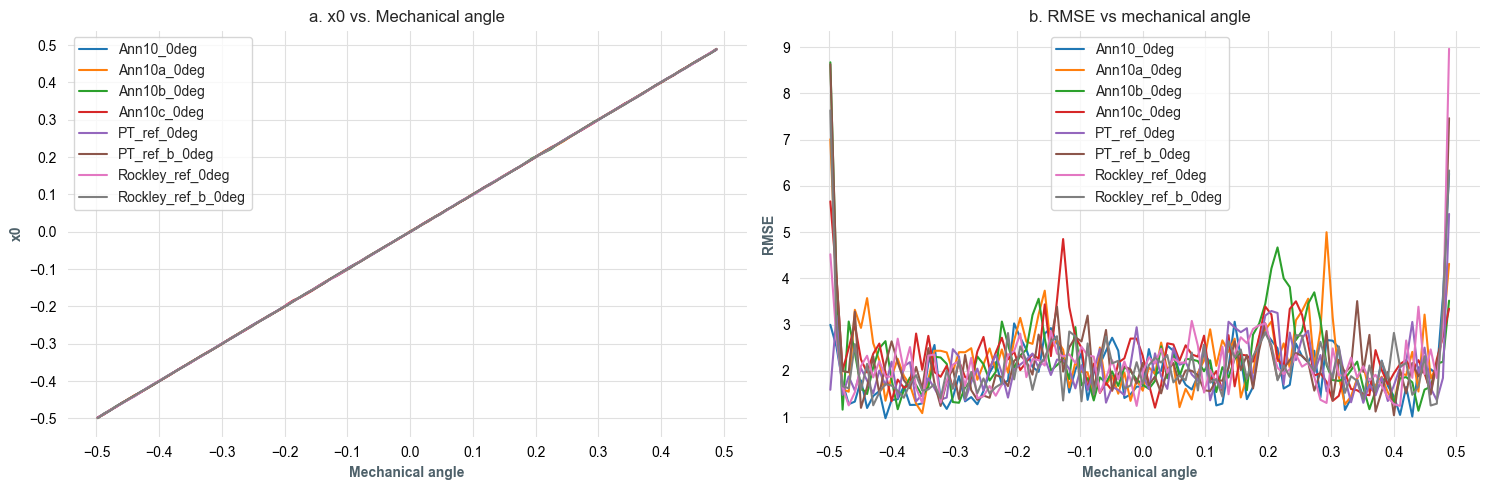
\includegraphics{notebooks/c_optimization_files/figure-pdf/fig-4-6-output-1.png}

}

\caption{\label{fig-4-6}Optimized RMSE for 0.1 nm Si wafers}

\end{figure}

The final result for RMSE shown in plot b represents the reference RMSE
calculated for very smooth wafers (0.1 nm). This error will be used to
compare with rougher samples. Notice that the RMSE increases for angles
greater than +-0.45 deg, so that RMSE parameter is valid only within
this range.

\newpage

\bookmarksetup{startatroot}

\hypertarget{rmse-roughness-characterization}{%
\chapter{RMSE-roughness
characterization}\label{rmse-roughness-characterization}}

The final step after having reconstructed base functions from smooth
samples (0.1 nm) and calculating a reference RMSE is to compare rougher
samples with respect to this. The roughness parameters are shown in
Table~\ref{tbl-2}. All the datasets were acquired along the on-axis at
+-20 deg and at 7 off-axis positions from -0.15 to 0.15 deg with 0.05
deg steps.

\hypertarget{tbl-2}{}
\begin{longtable}[]{@{}llll@{}}
\caption{\label{tbl-2}Roughness parameters}\tabularnewline
\toprule\noalign{}
& roughness (nm) & points & angle \\
file & & & \\
\midrule\noalign{}
\endfirsthead
\toprule\noalign{}
& roughness (nm) & points & angle \\
file & & & \\
\midrule\noalign{}
\endhead
\bottomrule\noalign{}
\endlastfoot
Ann10 & 0.11 & 4096 & 20 \\
PT\_ref & 0.13 & 4096 & 20 \\
Rockley\_ref & 0.10 & 4096 & 20 \\
Ann5 & 1.00 & 4096 & 20 \\
Ann7 & 0.97 & 4096 & 20 \\
PT\_3um & NaN & 4096 & 20 \\
Rockley\_rough & 315.00 & 4096 & 20 \\
Ann\_5min & NaN & 4096 & 20 \\
Ann\_4min & NaN & 4096 & 20 \\
Ann\_3min & NaN & 4096 & 20 \\
Ann\_2min & NaN & 4096 & 20 \\
Ann\_1min & NaN & 4096 & 20 \\
\end{longtable}

The roughness was measured using an atomic force microscope (afm) as
shown in Figure~\ref{fig-afm}

\begin{figure}

{\centering 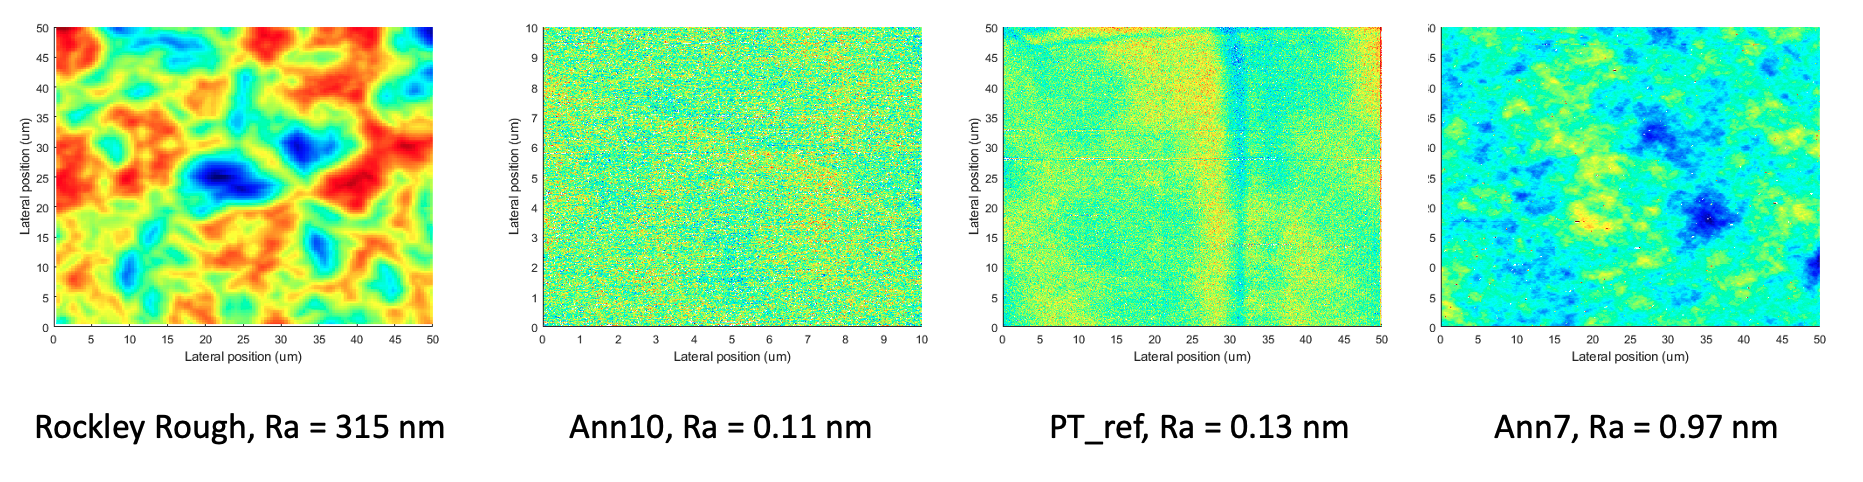
\includegraphics{notebooks/figures/d/afm.png}

}

\caption{\label{fig-afm}AFM measurements}

\end{figure}

\hypertarget{rmse-roughness-bands}{%
\section{RMSE-roughness bands}\label{rmse-roughness-bands}}

Figure~\ref{fig-5-1} shows RMSE-roughness characterization using
Rockley\_ref (0.1 nm) as a reference base function. Notice that there
are several bands representing different roughness levels.
Figure~\ref{fig-5-1} a shows three band levels for the different
roughness values including 0.1 nm, 1 nm and \(\mu m\). It is possible to
differentiate between 0.1 nm and 1 nm levels which is a limitation when
using only the Aq values. The 0.1 nm band is between 0 and 15 RMSE,
while the 1 nm is 35 and 50 RMSE.

Figure~\ref{fig-5-2} b shows the RMSE normalized with respect to the
amplitude correction factor and using a log scale. In this case the band
spacing is wider due to the log scale.

\begin{figure}

{\centering 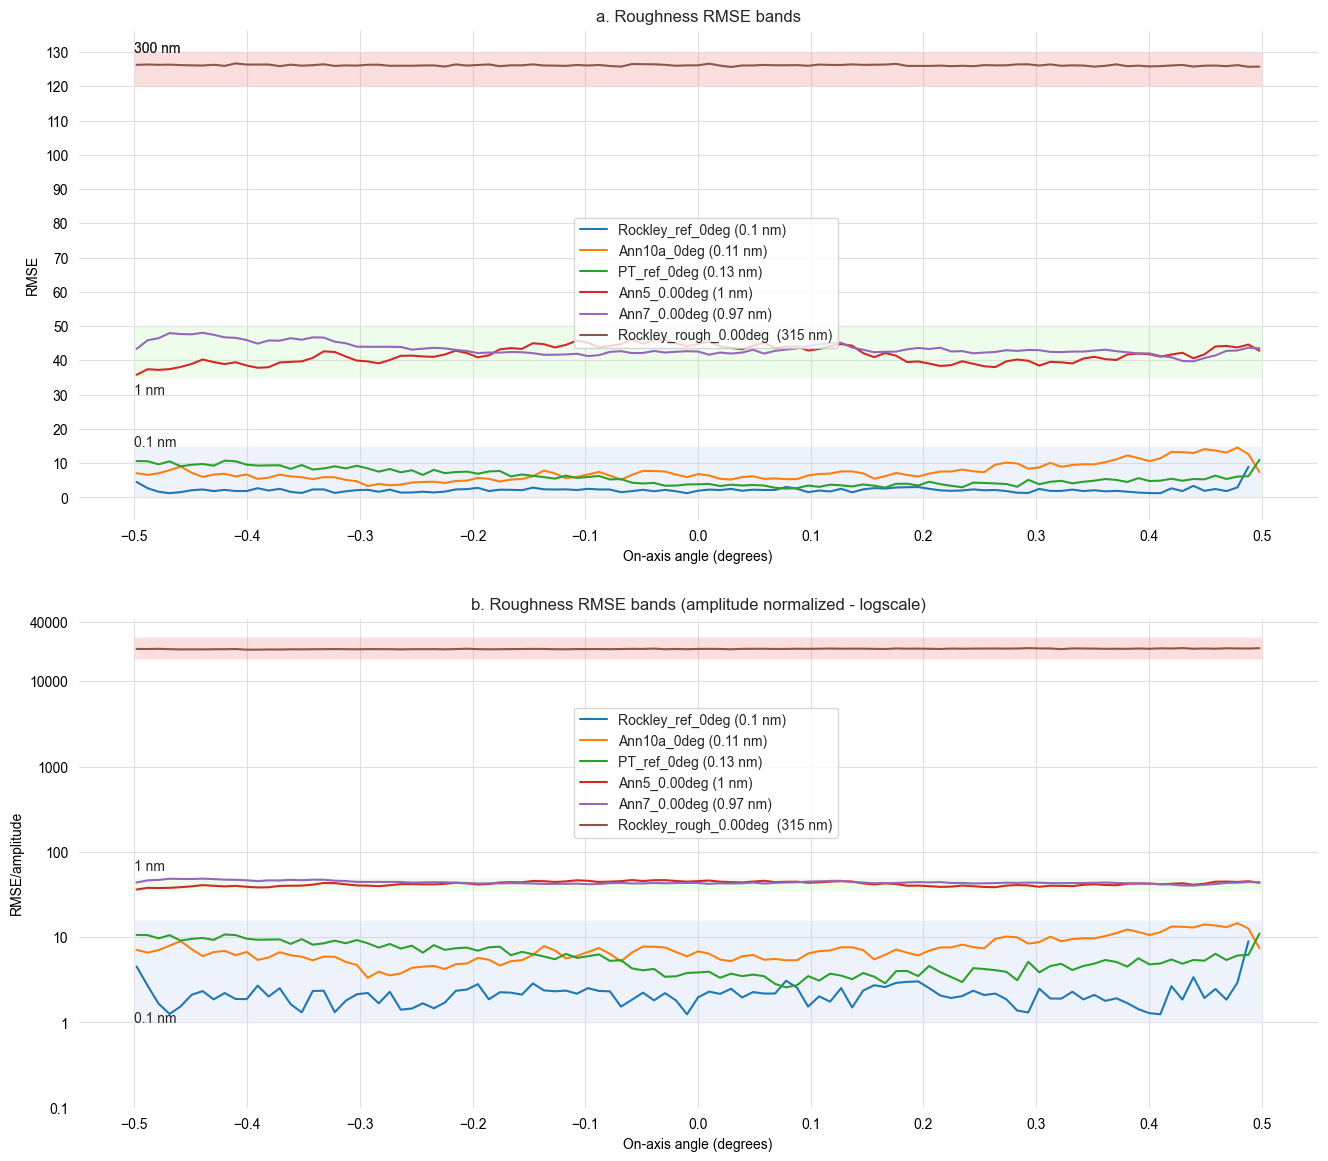
\includegraphics{notebooks/d_RMSE_files/figure-pdf/fig-5-1-output-1.png}

}

\caption{\label{fig-5-1}Roughness RMSE bands}

\end{figure}

A comparison of the same roughness values but using the Aq values is
shown in Figure~\ref{fig-5-2}. Notice the Aq values have a cosine shape
and the 0.1 nm and 1 nm bands are not clearly separated. This is because
for very smooth wafer the sampling points are limited over the main
curve, hence the Aq values are not very sensitive to roughness changes
in the nm scale. When focusing only in +-0.1 deg the Aq values seem to
have a band behaviour, however because of the very small Aq values the
resolution is too small to clearly distinguish between the different
roughness levels.

\begin{figure}

{\centering 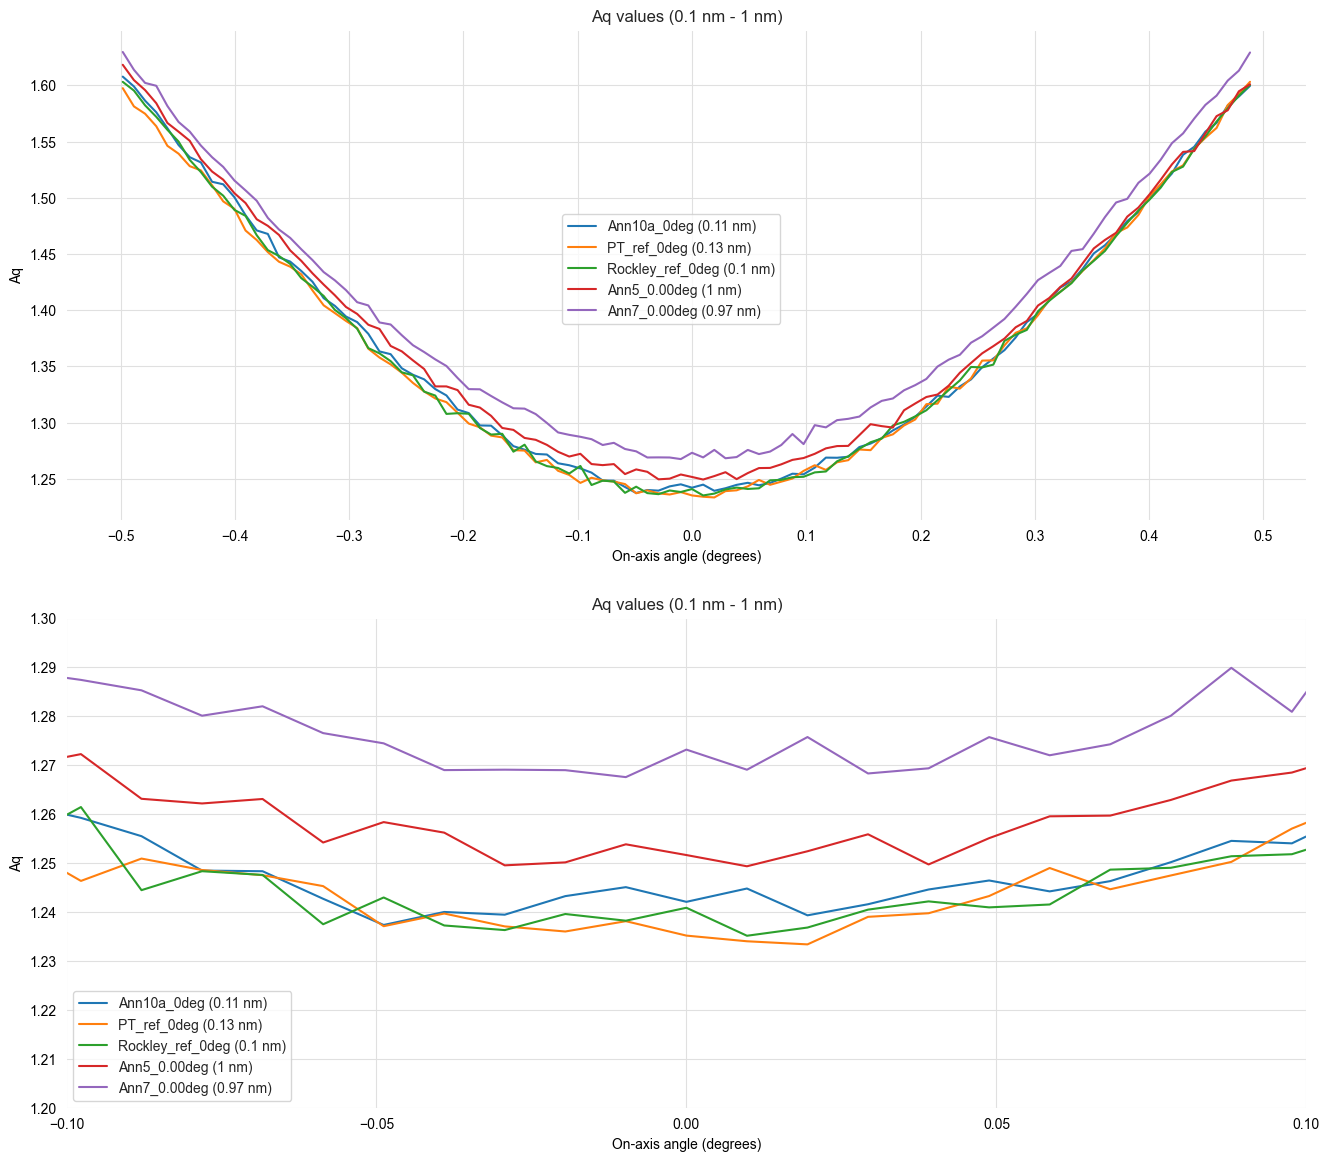
\includegraphics{notebooks/d_RMSE_files/figure-pdf/fig-5-2-output-1.png}

}

\caption{\label{fig-5-2}Aq values}

\end{figure}

\hypertarget{rmse-roughness-wafer-polishing}{%
\section{RMSE-roughness wafer
polishing}\label{rmse-roughness-wafer-polishing}}

Figure~\ref{fig-5-3} shows the relationship between roughness and
polishing time of a wafer. The more polishing time the smoother the
wafer becomes as expected. A time longer than 5 min is required to
obtain a roughness below 1 nm. With this propose methodology it is
possible to characterize different wafers after polishing and compare
them with respect to a reference wafer.

\begin{figure}

{\centering 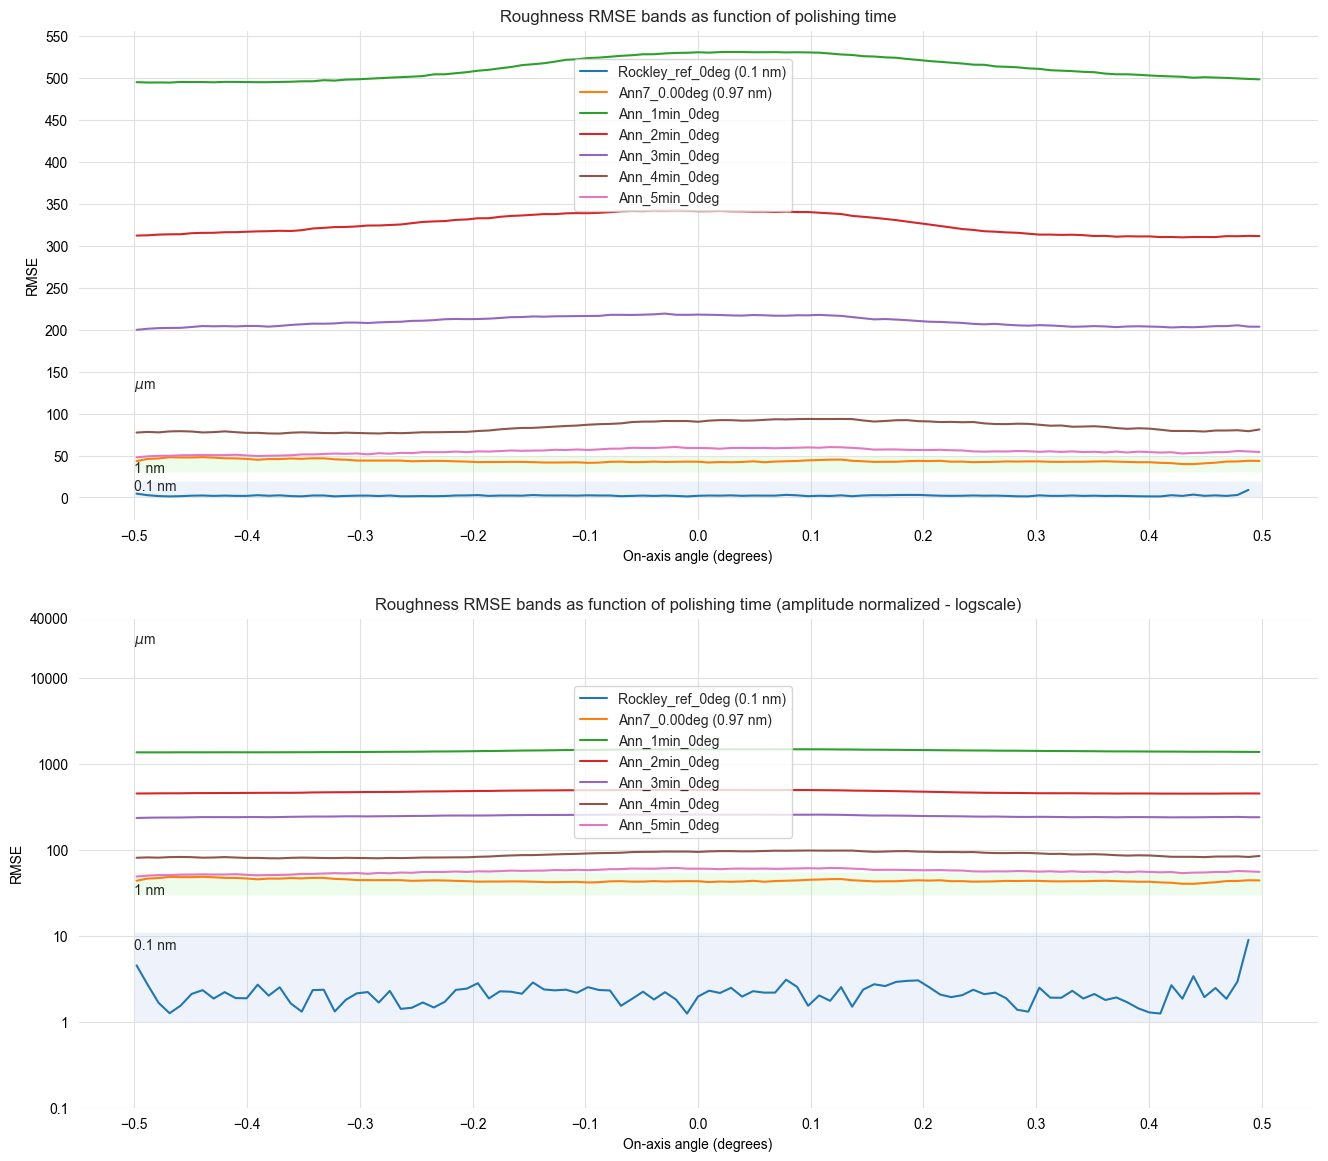
\includegraphics{notebooks/d_RMSE_files/figure-pdf/fig-5-3-output-1.png}

}

\caption{\label{fig-5-3}Roughness RMSE bands}

\end{figure}

\hypertarget{repeatability-and-data-conditions.}{%
\section{Repeatability and data
conditions.}\label{repeatability-and-data-conditions.}}

In order to know the requirements of the off-axis aligment different
off-axis datasets as the one shown in Figure~\ref{fig-3-9} were
acquired. The RMSE was then calculated using the same method. The
results are:

\begin{figure}

{\centering 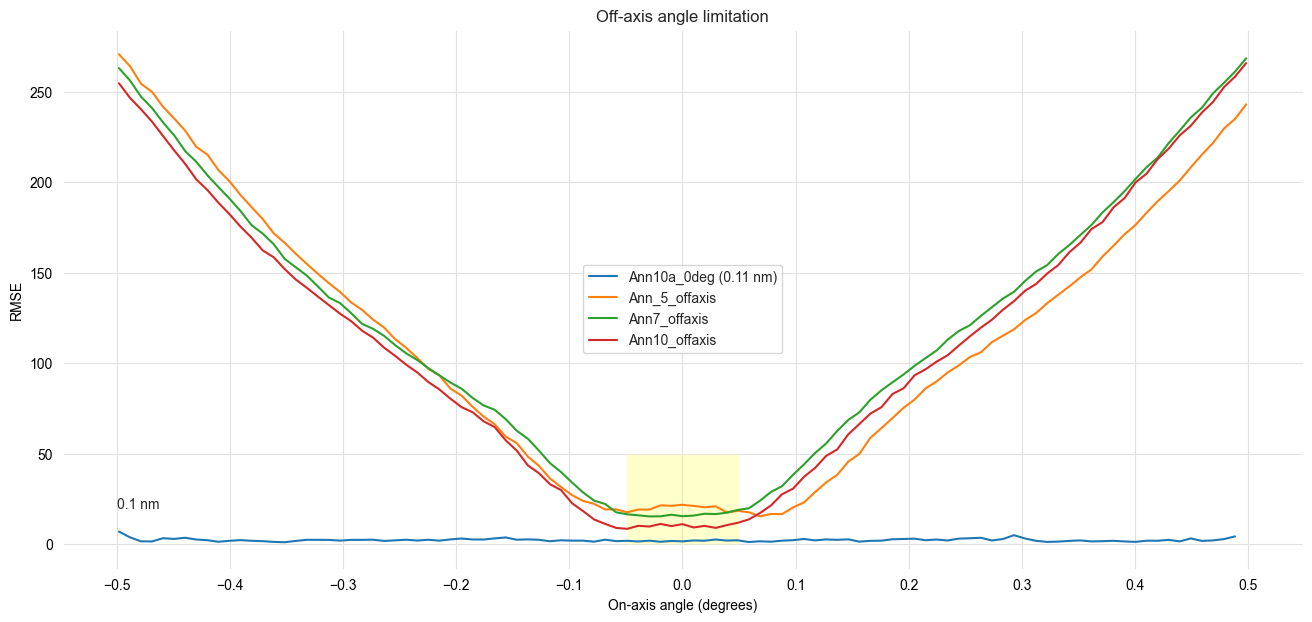
\includegraphics{notebooks/d_RMSE_files/figure-pdf/fig-5-4-output-1.png}

}

\caption{\label{fig-5-4}Off-axis angle limitations}

\end{figure}

In this case the results imply that the data needs to be collected at
off-axis positions withing +-0.05 deg in order to obtain reproducible
results. Notice outside this range the error increases significantly.
Hence, in practice there has to be a precise control over the scanning
angles using a vacuum in a clean room to make sure the data is collected
within the required scanning on-axis and off-axis angles. This
limitation is illustrated in Figure~\ref{fig-5-5} , in this case the
Ann10 wafer at 0 deg was used as the reference base function. Then the
same wafer was fit and the RMSE was calculated but at different off-axis
positions. Notice how the RMSE results are not consistent with the
reference base function.

\begin{figure}

{\centering 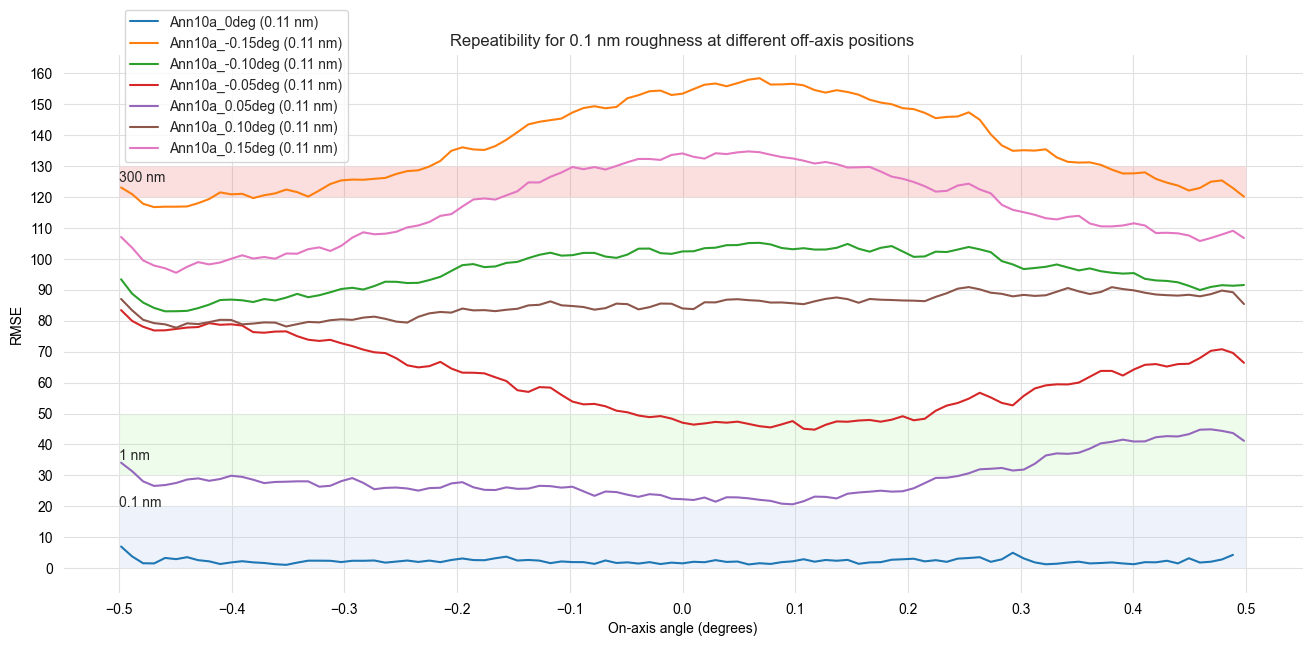
\includegraphics{notebooks/d_RMSE_files/figure-pdf/fig-5-5-output-1.png}

}

\caption{\label{fig-5-5}Repeatibility for 0.1 nm roughness at different
off-axis positions}

\end{figure}

A similar situation is illustrated in Figure~\ref{fig-5-6} , in this
case the Ann10a was used as a reference base function. Notice how the
orange curve is outside the 0.1 nm band. This is due to scratches/dust
in the wafer that can affect the roughness characterization. Hence, it
is important to have a clean wafer under control enviroments that can be
met in a controlled clean room.

\begin{figure}

{\centering 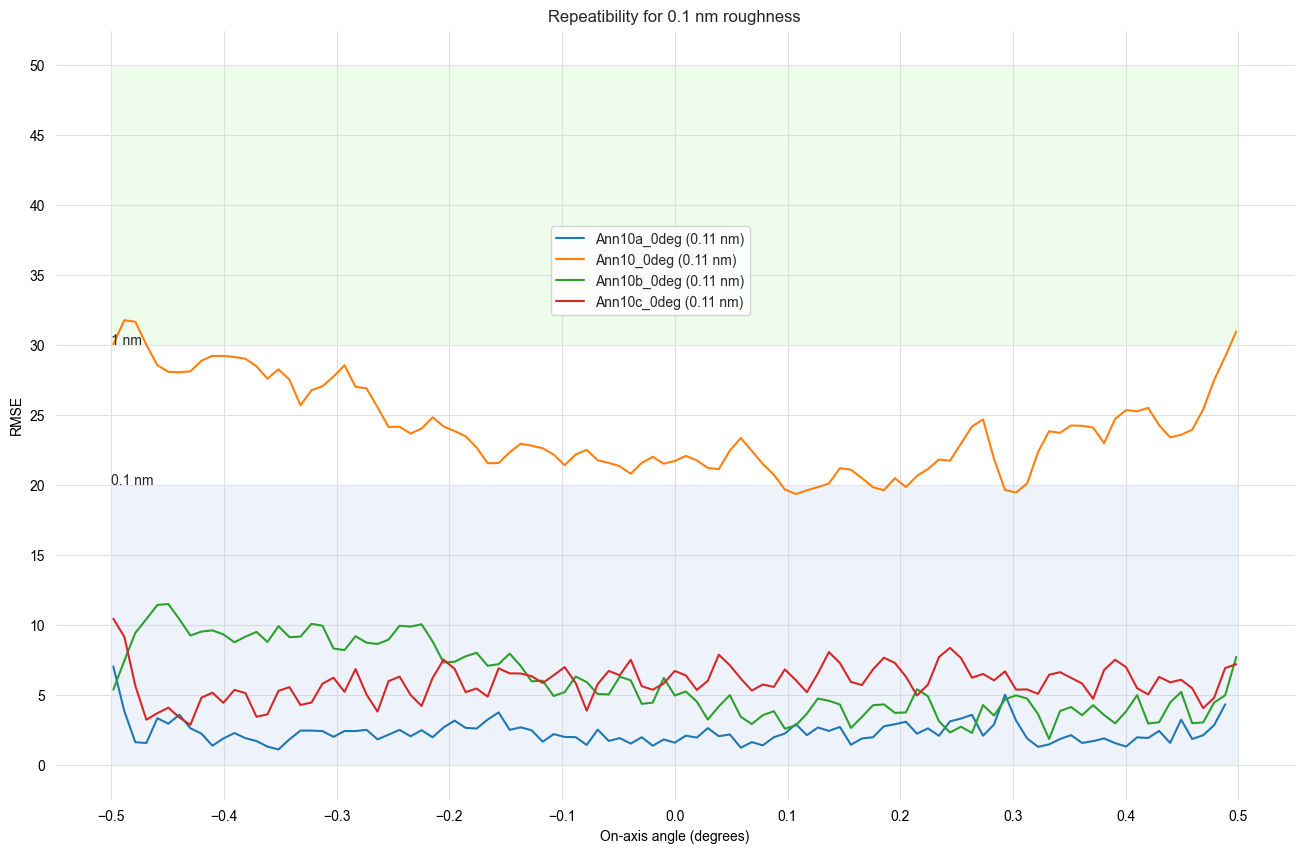
\includegraphics{notebooks/d_RMSE_files/figure-pdf/fig-5-6-output-1.png}

}

\caption{\label{fig-5-6}Repeatibility of RMSE roughness in the same
wafer}

\end{figure}

Finally when using a 0.1 nm wafer as a refence function at 0 deg
off-axis and fitting Ann 5 (1 nm) at different off-axis positions the
result is not repeatable. For different off-axis positions the RMSE is
not consistent and outside the expected 1 nm band. This is illustrated
in Figure~\ref{fig-5-7}.

\begin{figure}

{\centering 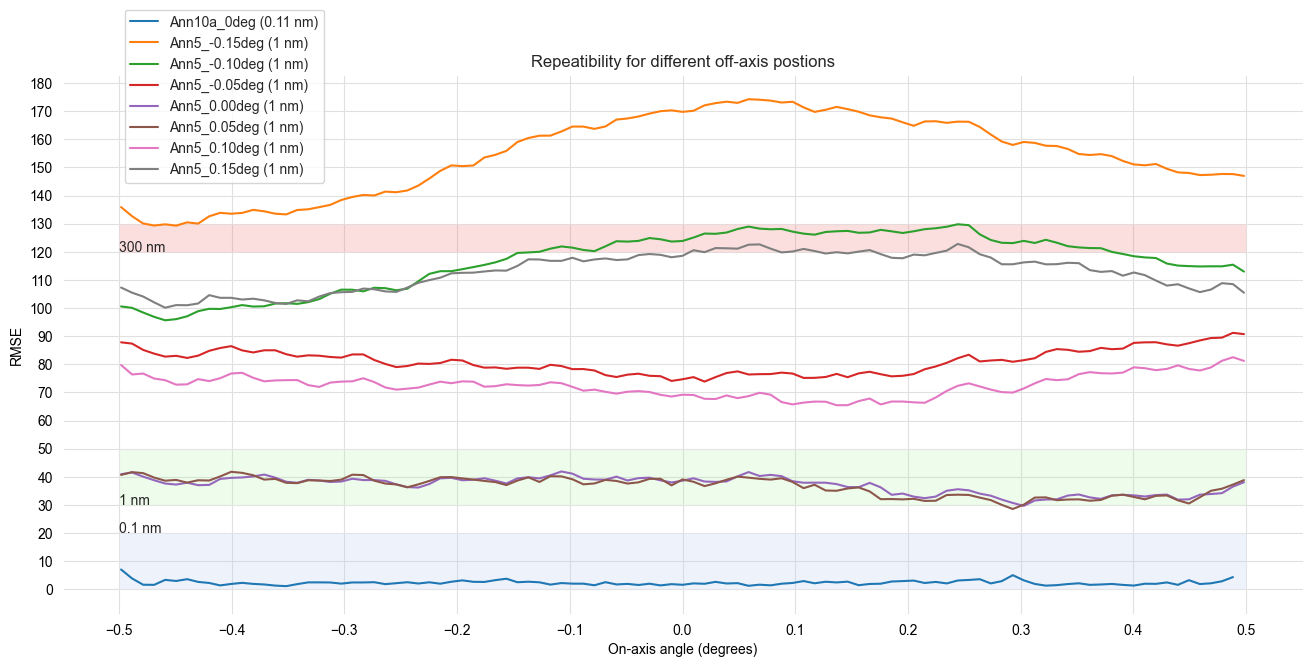
\includegraphics{notebooks/d_RMSE_files/figure-pdf/fig-5-7-output-1.png}

}

\caption{\label{fig-5-7}Repeatibility for 0.1 nm roughness at different
off-axis positions}

\end{figure}

According to \#knuth84 Knuth (1984)

\bookmarksetup{startatroot}

\hypertarget{conclusions}{%
\chapter{Conclusions}\label{conclusions}}

\begin{enumerate}
\def\labelenumi{\arabic{enumi}.}
\tightlist
\item
\item
\end{enumerate}

\bookmarksetup{startatroot}

\hypertarget{references}{%
\chapter*{References}\label{references}}
\addcontentsline{toc}{chapter}{References}

\markboth{References}{References}

\hypertarget{refs}{}
\begin{CSLReferences}{1}{0}
\leavevmode\vadjust pre{\hypertarget{ref-knuth84}{}}%
Knuth, Donald E. 1984. {``Literate Programming.''} \emph{Comput. J.} 27
(2): 97--111. \url{https://doi.org/10.1093/comjnl/27.2.97}.

\end{CSLReferences}



\end{document}
